\PassOptionsToPackage{unicode=true}{hyperref} % options for packages loaded elsewhere
\PassOptionsToPackage{hyphens}{url}
%
\documentclass[]{book}
\usepackage{lmodern}
\usepackage{amssymb,amsmath}
\usepackage{ifxetex,ifluatex}
\usepackage{fixltx2e} % provides \textsubscript
\ifnum 0\ifxetex 1\fi\ifluatex 1\fi=0 % if pdftex
  \usepackage[T1]{fontenc}
  \usepackage[utf8]{inputenc}
  \usepackage{textcomp} % provides euro and other symbols
\else % if luatex or xelatex
  \usepackage{unicode-math}
  \defaultfontfeatures{Ligatures=TeX,Scale=MatchLowercase}
\fi
% use upquote if available, for straight quotes in verbatim environments
\IfFileExists{upquote.sty}{\usepackage{upquote}}{}
% use microtype if available
\IfFileExists{microtype.sty}{%
\usepackage[]{microtype}
\UseMicrotypeSet[protrusion]{basicmath} % disable protrusion for tt fonts
}{}
\IfFileExists{parskip.sty}{%
\usepackage{parskip}
}{% else
\setlength{\parindent}{0pt}
\setlength{\parskip}{6pt plus 2pt minus 1pt}
}
\usepackage{hyperref}
\hypersetup{
            pdftitle={SHEDS Northeast Stream Temperature Model},
            pdfauthor={Jeff Walker, Ben Letcher, and Dan Hocking},
            pdfborder={0 0 0},
            breaklinks=true}
\urlstyle{same}  % don't use monospace font for urls
\usepackage{longtable,booktabs}
% Fix footnotes in tables (requires footnote package)
\IfFileExists{footnote.sty}{\usepackage{footnote}\makesavenoteenv{longtable}}{}
\usepackage{graphicx,grffile}
\makeatletter
\def\maxwidth{\ifdim\Gin@nat@width>\linewidth\linewidth\else\Gin@nat@width\fi}
\def\maxheight{\ifdim\Gin@nat@height>\textheight\textheight\else\Gin@nat@height\fi}
\makeatother
% Scale images if necessary, so that they will not overflow the page
% margins by default, and it is still possible to overwrite the defaults
% using explicit options in \includegraphics[width, height, ...]{}
\setkeys{Gin}{width=\maxwidth,height=\maxheight,keepaspectratio}
\setlength{\emergencystretch}{3em}  % prevent overfull lines
\providecommand{\tightlist}{%
  \setlength{\itemsep}{0pt}\setlength{\parskip}{0pt}}
\setcounter{secnumdepth}{5}
% Redefines (sub)paragraphs to behave more like sections
\ifx\paragraph\undefined\else
\let\oldparagraph\paragraph
\renewcommand{\paragraph}[1]{\oldparagraph{#1}\mbox{}}
\fi
\ifx\subparagraph\undefined\else
\let\oldsubparagraph\subparagraph
\renewcommand{\subparagraph}[1]{\oldsubparagraph{#1}\mbox{}}
\fi

% set default figure placement to htbp
\makeatletter
\def\fps@figure{htbp}
\makeatother

\usepackage{booktabs}
\usepackage{amsthm}
\makeatletter
\def\thm@space@setup{%
  \thm@preskip=8pt plus 2pt minus 4pt
  \thm@postskip=\thm@preskip
}
\makeatother
\usepackage[]{natbib}
\bibliographystyle{apalike}

\title{SHEDS Northeast Stream Temperature Model}
\author{\href{https://walkerenvres.com}{Jeff Walker}, \href{https://www.lsc.usgs.gov/?q=cafb-ben-letcher}{Ben Letcher}, and \href{https://hockinglab.weebly.com/}{Dan Hocking}}
\date{v1.3.0 (Sep 7, 2021)}

\begin{document}
\maketitle

{
\setcounter{tocdepth}{1}
\tableofcontents
}
\hypertarget{intro}{%
\chapter{Introduction}\label{intro}}

The SHEDS stream temperature model was developed to predict daily stream temperatures at both gaged and un-gaged catchments across the northeast U.S. based on geospatial characteristics and weather conditions.

The model is based on a linear mixed effects framework that accounts for spatial and temporal correlations using a hierachical Bayesian structure. \citet{Letcher2016} describe the initial development of this model framework, and apply it to a small region in western Massachusetts. See the \protect\hyperlink{model-overview}{Model Overview} section below for a brief introduction to the model, or the \protect\hyperlink{theory}{Theory} section a more detailed explanation.

The documentation is divided into the following sections:

\begin{enumerate}
\def\labelenumi{\arabic{enumi}.}
\tightlist
\item
  \protect\hyperlink{intro}{Introduction} : provides an overview the stream temperature model and documentation, as well as a snapshot of the current calibration
\item
  \protect\hyperlink{theory}{Theory} : describes how the model works including the underlying structure and theory
\item
  \protect\hyperlink{data-sources}{Data Sources} : describes the datasets used as inputs to the model
\item
  \protect\hyperlink{data-processing}{Data Processing} : describes how input datasets are processed prior to model fitting (i.e.~QAQC procedures)
\item
  \protect\hyperlink{calibration-and-validation}{Calibration and Validation} : describes how well the model predicts stream temperature based on observations that were included (calibration) and excluded (validation) from the model fitting process
\item
  \protect\hyperlink{predictions}{Predictions} : describes how predictions are generated after the model is calibrated and describes the various summary metrics that are computed for each catchment
\item
  \protect\hyperlink{download}{Download} : provides links to download the model predictions, catchment delineation (shapefiles), and covariates dataset.
\end{enumerate}

The model will be periodically updated and re-calibrated (approximately once every 6 months) to incorporate any new temperature observations, and to make any necessary revisions to the data processing and/or model structure. With each update, a new version will be assigned to the model, and this documentation website will be updated to reflect the most recent performance of the model. A brief summary of the changes associated with each new version is provided in the \protect\hyperlink{change-log}{Change Log} below.

\hypertarget{model-overview}{%
\section{Model Overview}\label{model-overview}}

The SHEDS stream temperature model predicts daily mean stream temperature based on geospatial characteristics and daily weather conditions. Predictions are made at a relatively fine spatial resolution based on a customized catchment delineation (average size about 2 km\textsuperscript{2}) across the northeast U.S. from Maine to Virginia. Predictions are limited to streams and rivers with drainage areas less than 200 km\textsuperscript{2}. Heavily impounded rivers are also excluded from the model.

The model uses a hierarchical Bayesian structure to account for spatial correlation in temperature between near-by locations through random effects for both the individual catchments and the larger watershed (HUC8) containing that catchment. Therefore, catchments within the same HUC8 watershed share a set of HUC-specific coefficients. Year to year variations in temperature are also accounted for using a random effect for the year.

\hypertarget{current-snapshot}{%
\section{Current Snapshot}\label{current-snapshot}}

Table \ref{tab:table-intro-gof} provides a snapshot of the calibration and validation performance for the current version of the model (v1.3.0). More details about the model performance can be found in the \protect\hyperlink{calibration-and-validation}{Calibration and Validation} section.

\begin{table}

\caption{\label{tab:table-intro-gof}Summary statistics of model calibration and validation}
\centering
\begin{tabular}[t]{l|r|r}
\hline
 & Calibration & Validation\\
\hline
\# Daily Observations & 749,327 & 85,228\\
\hline
\# Time Series & 8,495 & 959\\
\hline
\# Catchments & 3,077 & 614\\
\hline
\# HUC8s & 142 & 104\\
\hline
\# Years & 29.0 & 25.0\\
\hline
RMSE (degC) & 1.152 & 1.589\\
\hline
Mean Residual (degC) & 0.076 & 0.137\\
\hline
Median Residual (degC) & 0.087 & 0.150\\
\hline
Mean Absolute Residual (degC) & 0.866 & 1.148\\
\hline
Median Absolute Residual (degC) & 0.678 & 0.883\\
\hline
Minimum Residual (degC) & -12.129 & -15.074\\
\hline
1st Percentile Residual (degC) & -2.918 & -3.875\\
\hline
99th Percentile Residual (degC) & 2.944 & 4.215\\
\hline
Maximum Residual (degC) & 13.775 & 14.658\\
\hline
\end{tabular}
\end{table}

\hypertarget{model-versioning}{%
\section{Model Versioning}\label{model-versioning}}

The SHEDS stream temperature model uses semantic versioning of the form: \texttt{vX.Y.Z}

\begin{itemize}
\tightlist
\item
  \texttt{X} is the \textbf{major} version, which will be incremented when there is a major change to the model theory, code, or datasets.
\item
  \texttt{Y} is the \textbf{minor} version, which will be incremented when there is a new set of results due to changes in the model code, datasets, processing procedures, etc.
\item
  \texttt{Z} is the \textbf{patch} version, which will be incremented only when there is a change to the documentation or code that \emph{does not} yield different results.
\end{itemize}

\hypertarget{source-code}{%
\section{Source Code}\label{source-code}}

The source code for the model itself and this documentation is available in the Github repository \href{https://github.com/walkerjeffd/sheds-temp-model}{walkerjeffd/sheds-temp-model}. Each version of the model will be included under the list of \href{https://github.com/walkerjeffd/sheds-temp-model/releases}{Releases}.

\hypertarget{change-log}{%
\section{Change Log}\label{change-log}}

\begin{itemize}
\tightlist
\item
  \textbf{\href{https://ecosheds.org/models/stream-temperature/v1.3.0/}{v1.3.0 (Sep 7, 2021)}}\\
  Add 2020 daymet, revise data screening procedures, re-calibrate full model.
\item
  \textbf{\href{https://ecosheds.org/models/stream-temperature/v1.2.0/}{v1.2.0 (Jul 10, 2020)}}\\
  Add 2019 daymet, re-calibrate full model.
\item
  \textbf{\href{https://ecosheds.org/models/stream-temperature/v1.1.1/}{v1.1.1 (Jan 16, 2020)}}\\
  Add air temperature scenarios (+2, +4, +6 degC), and \# days \textgreater{}= 24.9 and 27 degC to prediction derived metrics.
\item
  \textbf{\href{https://ecosheds.org/models/stream-temperature/v1.1.0/}{v1.1.0 (Dec 2, 2019)}}\\
  Add 2018 daymet data, re-calibrated full model.
\item
  \textbf{\href{https://ecosheds.org/models/stream-temperature/v1.0.2/}{v1.0.2 (Mar 26, 2019)}}\\
  Update documentation, add \protect\hyperlink{download}{Download} section containing links to model predictions, catchment delineation, and covariates.
\item
  \textbf{\href{https://ecosheds.org/models/stream-temperature/v1.0.1/}{v1.0.1 (Dec 10, 2018)}}\\
  Update documentation, remove auto-correlation term from goodness-of-fit summaries
\item
  \textbf{\href{https://ecosheds.org/models/stream-temperature/v1.0.0/}{v1.0.0 (Oct 25, 2018)}}\\
  Re-calibrated model, and finished documentation.
\item
  \textbf{\href{https://ecosheds.org/models/stream-temperature/v0.9.2/}{v0.9.2 (Jul 6, 2018)}}\\
  Major updates to documentation (introduction, theory, calibration and validation sections).
\item
  \textbf{\href{https://ecosheds.org/models/stream-temperature/v0.9.1/}{v0.9.1 (Jun 6, 2018)}}\\
  Updates to model versioning and configuration framework, and minor updates to documentation (still incomplete).
\item
  \textbf{\href{https://ecosheds.org/models/stream-temperature/v0.9.0/}{v0.9.0 (May 30, 2018)}}\\
  Preliminary release of the new model framework and documentation.
\item
  \textbf{\href{https://conte-ecology.github.io/conteStreamTemperature_northeast/}{Previous Versions} (prior to 2018)}\\
  Previous versions of the stream temperature model can be found \href{https://conte-ecology.github.io/conteStreamTemperature_northeast/}{here}. That website is now deprecated, but will remain available for future reference. Beginning with v1.0.0 of the new framework and codebase, all model changes and results will be tracked and made available.
\end{itemize}

\hypertarget{theory}{%
\chapter{Theory}\label{theory}}

The stream temperature model is a nested hierarchical Bayesian model that predicts daily stream temperature based on catchment characteristics and climate conditions. An early version of this model can be found in \citet{Letcher2016}.

Daily mean stream temperature for each catchment is assumed to be a normally distributed random variable:

\[t_{h,c,y,d} \sim \mathcal{N}(\mu_{h,c,y,d},\sigma_{[t]})\]

where \(t_{h,c,y,d}\) is the mean stream temperature on day \(d\) within year \(y\) for catchment \(c\), which is located within HUC8 \(h\). This random variable is normally distributed with an expected mean \(\mu_{h,c,y,d}\) and standard deviation \(\sigma_{[t]}\).

The expected mean is computed as:

\[
\mu_{h,c,y,d} = \left \{ \begin{array}{l l}
  \omega_{h,c,y,d} + \delta_{h}(t_{h,c,y,d-1} - \omega_{h,c,y,d-1}) & \quad \text{for } t_{h,c,y,d-1} \text{ is real} \\
  \omega_{h,c,y,d} & \quad \text{for } t_{h,c,y,d-1} \text{ is not real}
  \end{array} \right.
\]

where \(\delta_h\) is an autoregressive {[}AR(1){]} coefficient and \(\omega_{h,c,y,d}\) is the expected temperature before accounting for temporal autocorrelation in the error structure.

The expected temperature is computed as a linear equation with four sets of terms:

\[\omega_{h,c,y,d} = X_{[0]} B_{[0]} + X_{h,c} B_{h,c} + X_{h} B_{h} + X_{y} B_{y}\]

where

\begin{itemize}
\tightlist
\item
  \(B_{[0]}\) is a vector of fixed effect coefficients
\item
  \(B_{h,c}\) is a vector of random effect coefficients for catchment \(c\)
\item
  \(B_{h}\) is a vector of random effect coefficients for HUC \(h\)
\item
  \(B_{y}\) is a vector of random effect coefficients for year \(y\)
\end{itemize}

Each of these vectors is multiplied by a corresponding matrix containing the corresponding predictor values (\(X\)) of each catchment \(c\) (located within HUC \(h\)) and on each day \(d\) (within year \(y\)).

\hypertarget{fixed-effects}{%
\section{Fixed Effects}\label{fixed-effects}}

The fixed effects are shared among all catchments within the model domain. They include the following terms:

\begin{longtable}[]{@{}ll@{}}
\toprule
Variable & Description\tabularnewline
\midrule
\endhead
\texttt{intercept} & Intercept\tabularnewline
\texttt{AreaSqKM} & Total Drainage Area (km2)\tabularnewline
\texttt{impoundArea} & Impounded Drainage Area (km2)\tabularnewline
\texttt{agriculture} & Agricultural Land Cover (\%)\tabularnewline
\texttt{devel\_hi} & High Development Land Cover (\%)\tabularnewline
\texttt{forest} & Riparian (200 ft Buffer) Forest Cover (\%)\tabularnewline
\texttt{prcp2} & 2-day Precipitation (mm)\tabularnewline
\texttt{prcp30} & 30-day Precipitation (mm)\tabularnewline
\bottomrule
\end{longtable}

The fixed effects also include the following interaction terms.

\begin{longtable}[]{@{}ll@{}}
\toprule
Interaction Term & Description\tabularnewline
\midrule
\endhead
\texttt{prcp2.da} & 2-day Precipitaation x Drainage Area\tabularnewline
\texttt{prcp30.da} & 30-day Precipitaation x Drainage Area\tabularnewline
\texttt{airTemp.da} & Air Temperature x Total Drainage Area\tabularnewline
\texttt{airTemp.impoundArea} & Air Temperature x Impounded Drainage Area\tabularnewline
\texttt{airTemp.agriculture} & Air Temperature x Agricultural Land Cover\tabularnewline
\texttt{airTemp.forest} & Air Temperature x Riparian (200 ft Buffer) Forest Cover\tabularnewline
\texttt{airTemp.devel\_hi} & Air Temperature x High Development Land Cover\tabularnewline
\texttt{airTemp.prcp2} & Air Temperature x 2-day Precipitation\tabularnewline
\texttt{airTemp.prcp30} & Air Temperature x 30-day Precipitation\tabularnewline
\texttt{airTemp.prcp2.da} & Air Temperature x 2-day Precipitation x Drainage Area\tabularnewline
\texttt{airTemp.prcp30.da} & Air Temperature x 30-day Precipitation x Drainage Area\tabularnewline
\bottomrule
\end{longtable}

\hypertarget{catchment-random-effects}{%
\section{Catchment Random Effects}\label{catchment-random-effects}}

The random effects for each catchment (\(c\)) include the following variables:

\begin{longtable}[]{@{}ll@{}}
\toprule
Variable & Description\tabularnewline
\midrule
\endhead
\texttt{intercept} & Intercept\tabularnewline
\texttt{airTemp} & Air Temperature (degC)\tabularnewline
\texttt{temp7p} & 7-day Mean Air Temperature (degC)\tabularnewline
\bottomrule
\end{longtable}

\hypertarget{huc-random-effects}{%
\section{HUC Random Effects}\label{huc-random-effects}}

The random effects for each HUC (\(h\)) include the following variables:

\begin{longtable}[]{@{}ll@{}}
\toprule
Variable & Description\tabularnewline
\midrule
\endhead
\texttt{intercept} & Intercept\tabularnewline
\texttt{airTemp} & Air Temperature (degC)\tabularnewline
\texttt{temp7p} & 7-day Mean Air Temperature (degC)\tabularnewline
\bottomrule
\end{longtable}

\hypertarget{year-random-effects}{%
\section{Year Random Effects}\label{year-random-effects}}

The random effects for each year (\(y\)) include the following variables:

\begin{longtable}[]{@{}ll@{}}
\toprule
Variable & Description\tabularnewline
\midrule
\endhead
\texttt{intercept} & Intercept\tabularnewline
\bottomrule
\end{longtable}

\hypertarget{data-sources}{%
\chapter{Data Sources}\label{data-sources}}

\hypertarget{covariate-datasets}{%
\section{Covariate Datasets}\label{covariate-datasets}}

\hypertarget{catchment-delineation}{%
\subsection{Catchment Delineation}\label{catchment-delineation}}

The stream temperature model uses the \href{https://conte-ecology.github.io/shedsGisData/}{National Hydrography Dataset High Resolution Delineation Version 2 (NHDHRDV2)} catchment delineation.

Shapefiles of the catchments can be downloaded from: \url{https://ecosheds.org/assets/nhdhrd/v2/}

The \texttt{spatial\_XX.zip} files contain pre-staged datasets for each HUC2 region (e.g.~spatial\_01.zip contains the catchments for the HUC2 region 01).

\hypertarget{climate-data}{%
\subsection{Climate Data}\label{climate-data}}

Daily air temperature and precipitation were obtained from the \href{https://daymet.ornl.gov/}{Daymet V3} gridded estimates of daily weather parameters for North America. The raw Daymet datasets (NetCDF4 files) were processed using the code in \href{https://github.com/walkerjeffd/sheds-daymet}{\texttt{walkerjeffd/sheds-daymet}}.

\hypertarget{geospatial-characteristics}{%
\subsection{Geospatial Characteristics}\label{geospatial-characteristics}}

Geospatial characteristics of each catchment were generated using the code in \href{https://github.com/Conte-Ecology/shedsGisData/tree/master/basinCharacteristics}{basinCharacteristics}. More information can be found on the \href{https://conte-ecology.github.io/shedsGisData/}{SHEDS GIS Data} page.

\hypertarget{stream-temperature-observations}{%
\section{Stream Temperature Observations}\label{stream-temperature-observations}}

Temperature observations extractd from the \href{http://db.ecosheds.org}{SHEDS Stream Temperature Database}, which contains data uploaded from numerous state and federal agencies, universities, and non-profit organizations.

\hypertarget{data-summary}{%
\subsection{Data Summary}\label{data-summary}}

The following table summarizes the number of monitoring stations, deployments, and total observations for each agency and organization.

\begin{tabular}{l|l|r|r|r}
\hline
Agency ID & Agency Description & \# Stations & \# Deployments & \# Observations\\
\hline
ARA & Ausable River Association & 18 & 9 & 275,493\\
\hline
ARWC & Androscoggin River Watershed Council & 44 & 18 & 629,831\\
\hline
BCDEPS & Baltimore County Department of Environmental Protection and Sustainability & 28 & 23 & 223,674\\
\hline
BSP & Baxter State Park & 166 & 10 & 2,496,265\\
\hline
CTDEEP & CT Department of Energy and Environmental Protection & 5,064 & 1,128 & 16,301,707\\
\hline
CTVOLMON & CT Volunteer Monitoring & 779 & 318 & 3,404,004\\
\hline
FRITSCHIE & Keith Fritschie, Dartmouth & 67 & 67 & 164,581\\
\hline
HAYDEN & Michael Hayden & 56 & 6 & 653,675\\
\hline
HBM & Houlton Band of Malisset & 1 & 1 & 5,025\\
\hline
HCSWCD & Hancock County Soil and Water Conservation District & 19 & 10 & 239,006\\
\hline
HMF & Hopkins Memorial Forest & 4 & 4 & 22,136\\
\hline
JMU & James Madison University & 7 & 7 & 20,477\\
\hline
MADEP & MA Department of Environmental Protection & 1,768 & 548 & 1,228,324\\
\hline
MAFW & MA Fish and Wildlife & 48 & 48 & 24,127\\
\hline
MAFW\_RQ & MA Division of Fish and Wildlife, Rebecca Quinones & 37 & 35 & 150,687\\
\hline
MBSS & Maryland Biological Stream Survey & 474 & 474 & 43,278\\
\hline
MEDEP & ME Department of Environmental Protection & 1,133 & 521 & 4,281,264\\
\hline
MEDMR & Maine Department of Marine Resources & 56 & 29 & 228,314\\
\hline
MEDOT & ME Department of Transportation & 3 & 3 & 85,848\\
\hline
MEIFW & ME Inland Fisheries and Wildlife & 217 & 127 & 3,798,765\\
\hline
ME\_MC & Midcoast Conservancy & 29 & 17 & 275,379\\
\hline
MRWC & Miller's River Watershed Council & 30 & 18 & 920,749\\
\hline
NHDES & NH Department of Environmental Services & 18 & 18 & 1,641\\
\hline
NHFG & NH Department of Fish and Game & 25 & 25 & 2,831\\
\hline
NJDEP & New Jersey Department of Environmental Protection & 8 & 8 & 35,904\\
\hline
NJDFW & NJ Dept of Environmental Protection, Div of Fish and Wildlife & 154 & 154 & 1,100,988\\
\hline
NOAA & National Oceanic and Atmospheric Administration & 274 & 29 & 1,142,388\\
\hline
NPS\_UDR & National Park Service, Upper Delaware River & 20 & 16 & 290,014\\
\hline
NYDEC & NY Department of Environmental Conservation & 1,011 & 419 & 2,999,485\\
\hline
OARS & OARS & 8 & 8 & 1,032,728\\
\hline
PINDNR & Penobscot Indian Nation Department of Natural Resources & 84 & 37 & 401,621\\
\hline
PSU & Plymouth State University & 134 & 117 & 17,964,253\\
\hline
RIDEM & Rhode Island Department of Environmental Management & 119 & 85 & 239,019\\
\hline
SRBC & Susquehanna River Basin Commission & 351 & 60 & 18,926,101\\
\hline
SRCC & Saco River Corridor Commission & 8 & 8 & 8,927\\
\hline
SVWA & Southeastern Vermont Watershed Alliance & 5 & 5 & 99,417\\
\hline
TNC\_NJ & The Nature Conservancy, New Jersey & 14 & 14 & 774,921\\
\hline
TU\_ADK & Trout Unlimited, Adirondacks & 62 & 61 & 170,416\\
\hline
TU\_AF & Trout Unlimited, Art Flick Chapter & 22 & 8 & 150,135\\
\hline
TU\_CLEARWATER & Trout Unlimited, Clearwater Chapter & 38 & 24 & 136,693\\
\hline
TU\_DW & Trout Unlimited, Deerfield Watershed & 29 & 11 & 289,641\\
\hline
TU\_HR & Trout Unlimited, Housatonic River & 7 & 2 & 20,497\\
\hline
TU\_KV & Trout Unlimited, Kennebec Valley & 13 & 13 & 67,271\\
\hline
TU\_MMB & Trout Unlimited, Merry Meeting Bay & 62 & 20 & 896,381\\
\hline
TU\_NJ & Trout Unlimited, New Jersey Chapter & 61 & 61 & 555,272\\
\hline
TU\_NY & Trout Unlimited, New York Chapter & 43 & 43 & 111,284\\
\hline
UMAINE & University of Maine & 12 & 6 & 112,100\\
\hline
UMASS\_USGS & UMass USGS Cooperative Unit & 397 & 179 & 19,991,386\\
\hline
UNITY & Unity College & 8 & 4 & 263,184\\
\hline
USFS & US Forest Service & 518 & 136 & 6,135,136\\
\hline
USFS\_SRS & US Forest Service Southern Research Station & 8 & 8 & 40,983\\
\hline
USFWS\_LGL & US Fish and Wildlife Service, Lower Great Lakes FWCO & 11 & 11 & 59,232\\
\hline
USFWS\_ME & US Fish and Wildlife Service, Maine Field Office & 449 & 324 & 12,989,371\\
\hline
USFWS\_MNWR & US Fish and Wildlife Service, Moosehorn National Wildlife Refuge & 16 & 15 & 86,657\\
\hline
USGS & U.S. Geological Survey & 310 & 57 & 3,965,147\\
\hline
USGS\_BRD & US Geological Survey BRD & 11 & 11 & 11,421\\
\hline
USGS\_Conte & USGS Conte Lab & 129 & 33 & 2,623,727\\
\hline
USGS\_Leetown & USGS Leetown Science Center & 115 & 114 & 457,000\\
\hline
VAHUDY & VA HUDY & 33 & 33 & 136,266\\
\hline
VTFWD & VT Fish and Wildlife Department & 489 & 421 & 3,549,632\\
\hline
WVDNR & WV Department of Natural Resources & 214 & 214 & 835,882\\
\hline
\end{tabular}

\hypertarget{data-processing}{%
\chapter{Data Processing}\label{data-processing}}

A series of automated data screening and QA/QC procedures are used to process the raw stream temperature observations, and generate the final input dataset of mean daily stream temperatures, which is then used to calibrate and validate the model.

Processing of the raw stream temperature observations involves the following steps:

\begin{enumerate}
\def\labelenumi{\arabic{enumi}.}
\tightlist
\item
  Screen monitoring stations based on location and drainage area characteristics
\item
  Aggregate instantaneous observations to daily time steps
\item
  Screen daily mean temperature values and time series according to various QA/QC tests
\item
  Aggregate daily time series measured at multiple stations within a single catchment
\item
  Screen time series to exclude cold weather conditions when air temperature and water temperature are de-coupled
\item
  Split the final dataset into subsets for calibration (90\% of time series) and validation (10\% of time series)
\end{enumerate}

\hypertarget{screen-monitoring-stations}{%
\section{Screen Monitoring Stations}\label{screen-monitoring-stations}}

The full set of monitoring stations are first screened to exclude those that meet the following criteria:

\begin{enumerate}
\def\labelenumi{\arabic{enumi}.}
\tightlist
\item
  Located within 100 m of an impoundment
\item
  Located within a tidal zone
\item
  Located within a catchment having a drainage area greater than 200 sq km
\item
  Located within a catchment having a drainage area with greater than 50\% coverage by open water or wetlands
\end{enumerate}

\hypertarget{screen-daily-mean-values}{%
\section{Screen Daily Mean Values}\label{screen-daily-mean-values}}

After screening for the monitoring stations, the remaining time series are screened according to the following criteria:

\begin{enumerate}
\def\labelenumi{\arabic{enumi}.}
\tightlist
\item
  Remove daily values that have user-defined flag stored in the database
\item
  Remove daily values with mean temp \textless{} -25 degC
\item
  Remove daily values with mean or max temp \textgreater{} 35 degC
\item
  Remove time series with a high correlation between daily mean water and air temperature, which are suspected to be measurements of air temperature
\item
  Remove time series with fewer than 5 days of observations
\item
  Remove first and/or last day of each timeseries if the number of observations on those days is less than the median number of observations per day for the whole series (i.e.~the first and/or last day are incomplete)
\end{enumerate}

\hypertarget{combine-overlapping-timeseries}{%
\section{Combine Overlapping Timeseries}\label{combine-overlapping-timeseries}}

If there are two or more overlapping time series at a single monitoring station, then those time series are combined by:

\begin{enumerate}
\def\labelenumi{\arabic{enumi}.}
\tightlist
\item
  Compute the overall mean value on each date of the overlapping time series.
\item
  Remove any daily values having more than one time series and a difference in mean observed temperature greater than 5 deg C between those time series
\end{enumerate}

\hypertarget{screen-multiple-locations-within-single-catchment}{%
\section{Screen Multiple Locations within Single Catchment}\label{screen-multiple-locations-within-single-catchment}}

If there are multiple stations within a single catchment, then only one station is retained to represent that catchment based on the following criteria:

\begin{enumerate}
\def\labelenumi{\arabic{enumi}.}
\tightlist
\item
  Exclude stations located more than 60 m from the main flowline of the catchment
\item
  If more than one station remains, choose the stations with greatest number of observations between April and October
\item
  If more than one station still remains, choose the station located nearest to the pour point of the catchment
\end{enumerate}

\hypertarget{remove-cold-weather-periods}{%
\section{Remove Cold Weather Periods}\label{remove-cold-weather-periods}}

Lastly, each time series are truncated to the seasonal period during which water temperature and air temperature are coupled to exclude observations during cold weather periods.

\hypertarget{split-dataset-for-calibration-and-validation}{%
\section{Split Dataset for Calibration and Validation}\label{split-dataset-for-calibration-and-validation}}

The final dataset of mean daily stream temperature observations are then split for calibration and validation. The split is performed by randomly selecting 90\% of the time series for calibration, and using the remaining 10\% for validation.

\hypertarget{calibration-and-validation}{%
\chapter{Calibration and Validation}\label{calibration-and-validation}}

After processing all of the data, the model was fitted using jags. The observation dataset was split into 80\% for calibration, 20\% for validation.

\hypertarget{parameter-estimates}{%
\section{Parameter Estimates}\label{parameter-estimates}}

\hypertarget{fixed-effects-1}{%
\subsection{Fixed Effects}\label{fixed-effects-1}}

Figure \ref{fig:plot-params-fixed} and Table \ref{tab:table-params-fixed} present the estimated mean and 95\% credible region interval (CRI) of each fixed effect parameter. The intercept term is not shown in the figure because the values are much larger than the other parameters, and would thus skew the scale.

\begin{figure}
\centering
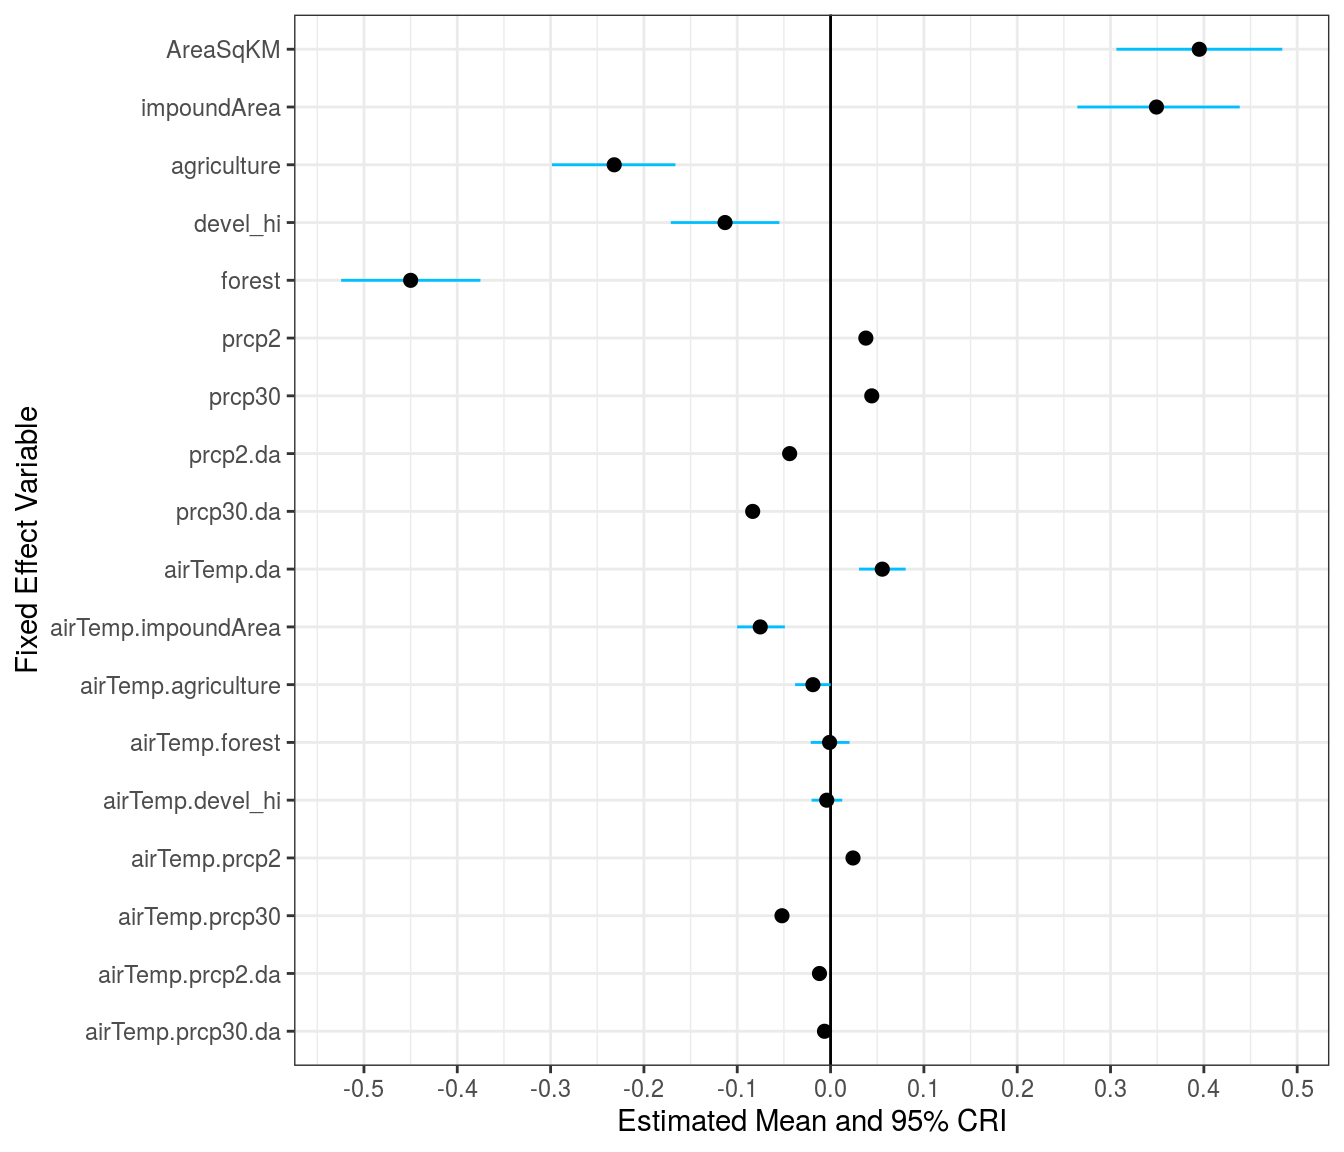
\includegraphics{sheds-temp-model_files/figure-latex/plot-params-fixed-1.pdf}
\caption{\label{fig:plot-params-fixed}Estimated Mean and 95\% CRI of Fixed Effects}
\end{figure}

\textbackslash{}begin\{table\}

\textbackslash{}caption\{\label{tab:table-params-fixed}Estimated Mean and 95\% CRI of Fixed Effects\}
\centering

\begin{tabular}[t]{l|r|r|r}
\hline
Variable & Mean & Lower CRI & Upper CRI\\
\hline
intercept & 16.833421530 & 16.67617588 & 16.9867338349\\
\hline
AreaSqKM & 0.395116342 & 0.30627141 & 0.4840870247\\
\hline
impoundArea & 0.349202949 & 0.26441219 & 0.4384439730\\
\hline
agriculture & -0.231818023 & -0.29860379 & -0.1662348226\\
\hline
devel\_hi & -0.113091616 & -0.17117577 & -0.0548478596\\
\hline
forest & -0.449975232 & -0.52445930 & -0.3751637908\\
\hline
prcp2 & 0.037811292 & 0.03591343 & 0.0395934936\\
\hline
prcp30 & 0.044143933 & 0.03778849 & 0.0505761489\\
\hline
prcp2.da & -0.043839749 & -0.04582635 & -0.0418767171\\
\hline
prcp30.da & -0.083451495 & -0.09003666 & -0.0767409762\\
\hline
airTemp.da & 0.055426531 & 0.03046611 & 0.0804564704\\
\hline
airTemp.impoundArea & -0.075351885 & -0.10018257 & -0.0489819699\\
\hline
airTemp.agriculture & -0.018888556 & -0.03803921 & 0.0001204872\\
\hline
airTemp.forest & -0.001042650 & -0.02127786 & 0.0203067821\\
\hline
airTemp.devel\_hi & -0.004110505 & -0.02032762 & 0.0124983349\\
\hline
airTemp.prcp2 & 0.024049145 & 0.02223997 & 0.0257588483\\
\hline
airTemp.prcp30 & -0.052055111 & -0.05564053 & -0.0485377100\\
\hline
airTemp.prcp2.da & -0.011881446 & -0.01361107 & -0.0101528157\\
\hline
airTemp.prcp30.da & -0.006500592 & -0.01012480 & -0.0029489054\\
\hline
\end{tabular}

\textbackslash{}end\{table\}

\hypertarget{huc8-random-effects}{%
\subsection{HUC8 Random Effects}\label{huc8-random-effects}}

Figure \ref{fig:plot-params-huc8} shows the estimated mean and 95\% credible region interval (CRI) for each random effect and HUC8. Table \ref{tab:table-params-huc8} lists the estimated mean and 95\% CRI of each parameter averaged over all HUC8s (mean value with standard deviation in parentheses).

\begin{figure}
\centering
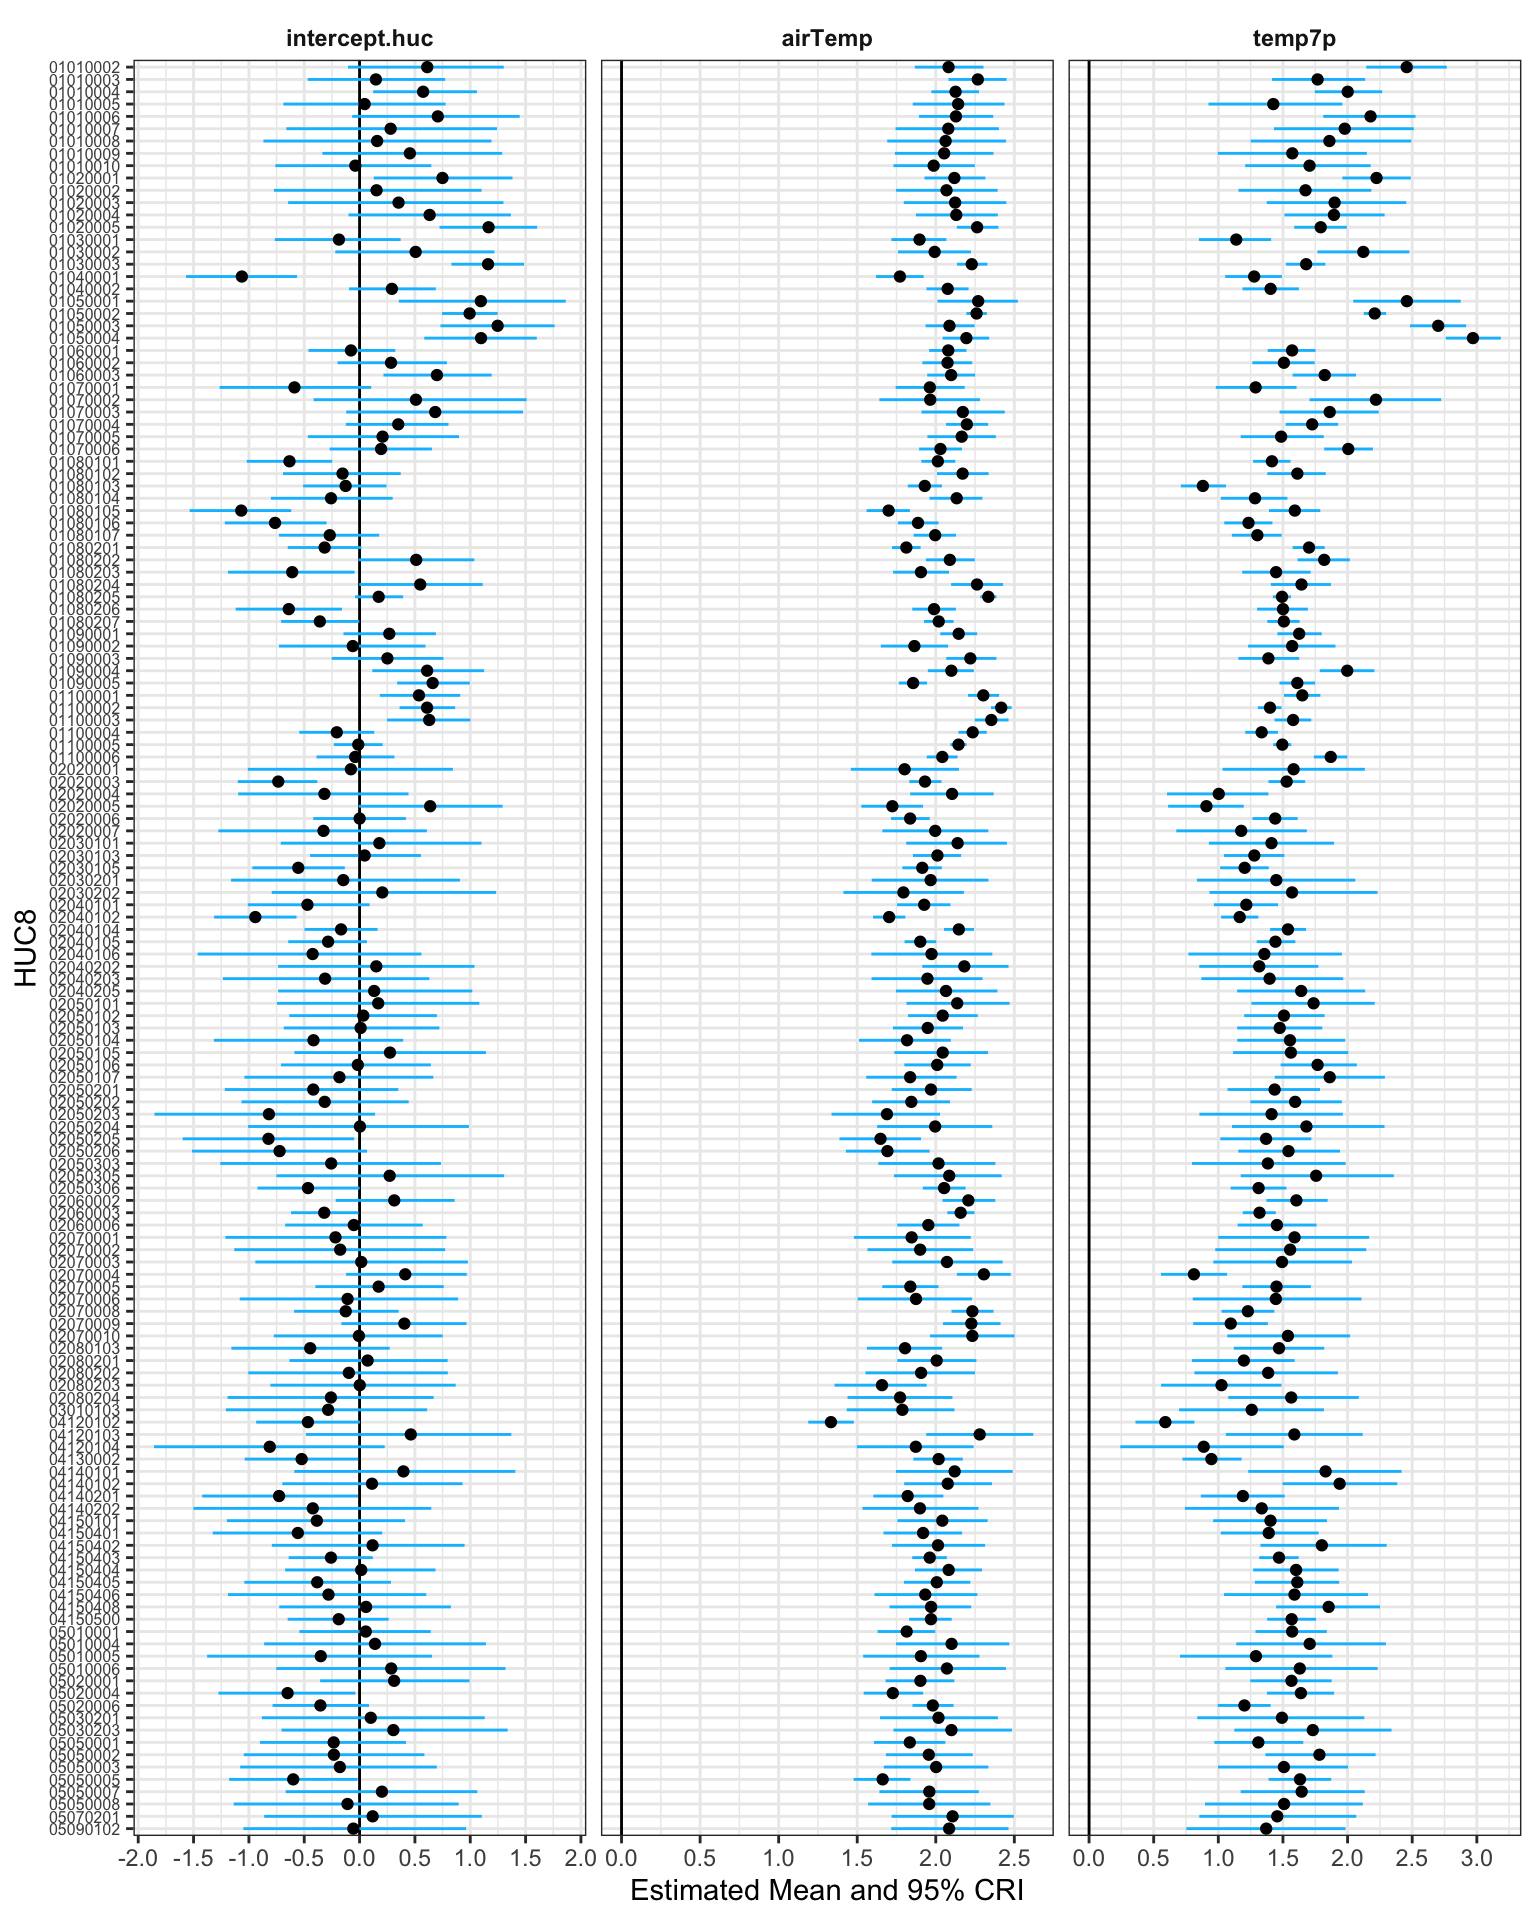
\includegraphics{sheds-temp-model_files/figure-latex/plot-params-huc8-1.pdf}
\caption{\label{fig:plot-params-huc8}Estimated Mean and 95\% CRI of HUC Random Effects for Each HUC8}
\end{figure}

\textbackslash{}begin\{table\}

\textbackslash{}caption\{\label{tab:table-params-huc8}Mean and 95\% CRI of HUC8 Random Effects Averaged Over All HUC8s (Mean Value and Std. Dev. in Parentheses)\}
\centering

\begin{tabular}[t]{l|r|r|r|r}
\hline
Variable & Count & Mean & Lower CRI & Upper CRI\\
\hline
intercept.huc & 142 & -0.001 (0.475) & -0.764 (0.537) & 0.764 (0.550)\\
\hline
airTemp & 142 & 1.989 (0.185) & 1.736 (0.224) & 2.241 (0.206)\\
\hline
temp7p & 142 & 1.434 (0.321) & 1.065 (0.362) & 1.803 (0.368)\\
\hline
\end{tabular}

\textbackslash{}end\{table\}

\hypertarget{catchment-random-effects-1}{%
\subsection{Catchment Random Effects}\label{catchment-random-effects-1}}

Figure \ref{fig:plot-params-catchment} shows the distribution of the estimated mean for each random effect term over all catchments. CRIs are not shown due to the large number of individual catchments (9231). Table \ref{tab:table-params-catchment} lists the estimated mean and 95\% CRI of each parameter averaged over all catchments (mean value with standard deviation in parentheses).

\begin{figure}
\centering
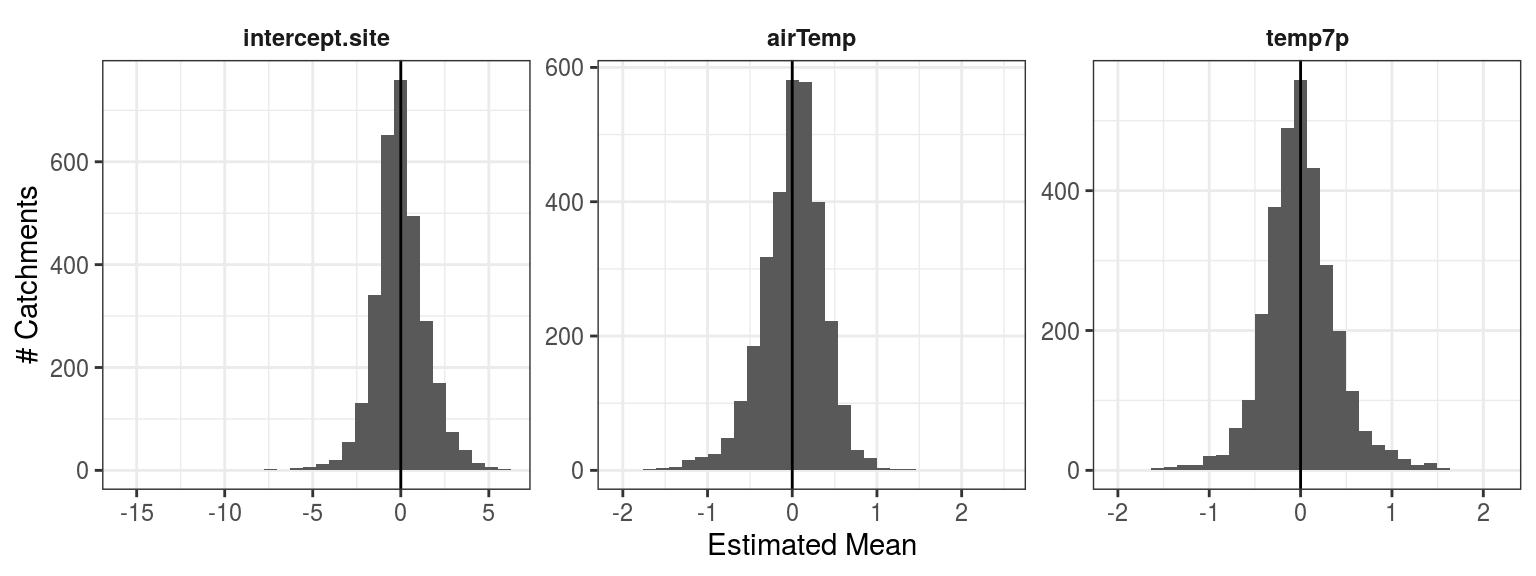
\includegraphics{sheds-temp-model_files/figure-latex/plot-params-catchment-1.pdf}
\caption{\label{fig:plot-params-catchment}Distribution of estimated mean for each random effect over all catchments}
\end{figure}

\textbackslash{}begin\{table\}

\textbackslash{}caption\{\label{tab:table-params-catchment}Estimated mean and 95\% CRI for each random effect averaged over all catchments (mean value with std. dev. in parentheses)\}
\centering

\begin{tabular}[t]{l|r|r|r|r}
\hline
Variable & Count & Mean & Lower CRI & Upper CRI\\
\hline
intercept.site & 3,077 & 0.001 (1.477) & -0.799 (1.488) & 0.800 (1.509)\\
\hline
airTemp & 3,077 & -0.000 (0.370) & -0.300 (0.381) & 0.300 (0.389)\\
\hline
temp7p & 3,077 & 0.000 (0.394) & -0.528 (0.467) & 0.529 (0.400)\\
\hline
\end{tabular}

\textbackslash{}end\{table\}

\hypertarget{year-random-effects-1}{%
\subsection{Year Random Effects}\label{year-random-effects-1}}

Figure \ref{fig:plot-params-year} and Table \ref{tab:table-params-year} present the mean and 95\% CRI of the intercept term for each year. Recall that there are no random effects for years other than the intercept.

\begin{figure}
\centering
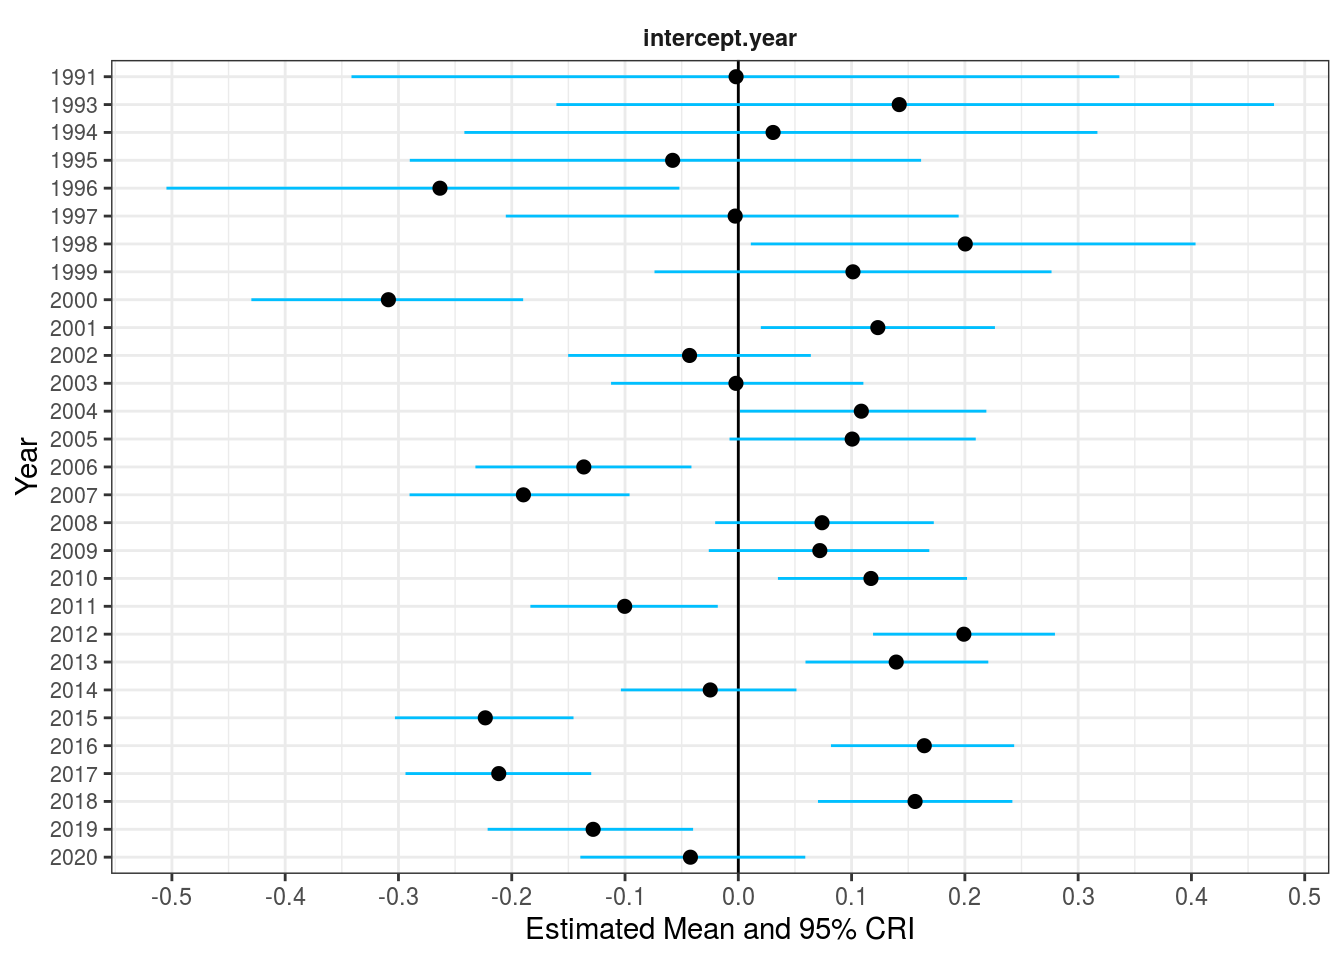
\includegraphics{sheds-temp-model_files/figure-latex/plot-params-year-1.pdf}
\caption{\label{fig:plot-params-year}Estimated Mean and 95\% CRI of Intercept Random Effect for Each Year}
\end{figure}

\textbackslash{}begin\{table\}

\textbackslash{}caption\{\label{tab:table-params-year}Estimated Mean and 95\% CRI of Intercept Random Effect for Each Year\}
\centering

\begin{tabular}[t]{l|r|r|r}
\hline
Year & Mean & Lower CRI & Upper CRI\\
\hline
1991 & -0.002 & -0.341 & 0.336\\
\hline
1993 & 0.142 & -0.161 & 0.473\\
\hline
1994 & 0.031 & -0.242 & 0.317\\
\hline
1995 & -0.058 & -0.290 & 0.161\\
\hline
1996 & -0.263 & -0.505 & -0.052\\
\hline
1997 & -0.003 & -0.205 & 0.195\\
\hline
1998 & 0.200 & 0.011 & 0.404\\
\hline
1999 & 0.101 & -0.074 & 0.277\\
\hline
2000 & -0.309 & -0.430 & -0.190\\
\hline
2001 & 0.123 & 0.020 & 0.227\\
\hline
2002 & -0.043 & -0.150 & 0.064\\
\hline
2003 & -0.002 & -0.112 & 0.110\\
\hline
2004 & 0.109 & 0.001 & 0.219\\
\hline
2005 & 0.101 & -0.008 & 0.210\\
\hline
2006 & -0.136 & -0.232 & -0.041\\
\hline
2007 & -0.190 & -0.290 & -0.096\\
\hline
2008 & 0.074 & -0.020 & 0.173\\
\hline
2009 & 0.072 & -0.026 & 0.169\\
\hline
2010 & 0.117 & 0.035 & 0.202\\
\hline
2011 & -0.100 & -0.184 & -0.018\\
\hline
2012 & 0.199 & 0.119 & 0.280\\
\hline
2013 & 0.139 & 0.059 & 0.221\\
\hline
2014 & -0.025 & -0.104 & 0.051\\
\hline
2015 & -0.223 & -0.303 & -0.145\\
\hline
2016 & 0.164 & 0.082 & 0.244\\
\hline
2017 & -0.211 & -0.294 & -0.130\\
\hline
2018 & 0.156 & 0.070 & 0.242\\
\hline
2019 & -0.128 & -0.221 & -0.040\\
\hline
2020 & -0.042 & -0.139 & 0.059\\
\hline
\end{tabular}

\textbackslash{}end\{table\}

\hypertarget{goodness-of-fit}{%
\section{Goodness-of-Fit}\label{goodness-of-fit}}

\hypertarget{all-observations}{%
\subsection{All Observations}\label{all-observations}}

Table \ref{tab:table-gof} summarizes the model goodness-of-fit for all observations in the calibration and validation datasets.

\begin{table}

\caption{\label{tab:table-gof}Summary statistics of model calibration and validation}
\centering
\begin{tabular}[t]{l|r|r}
\hline
 & Calibration & Validation\\
\hline
\# Daily Observations & 749,327 & 85,228\\
\hline
\# Time Series & 8,495 & 959\\
\hline
\# Catchments & 3,077 & 614\\
\hline
\# HUC8s & 142 & 104\\
\hline
\# Years & 29.0 & 25.0\\
\hline
RMSE (degC) & 1.152 & 1.589\\
\hline
Mean Residual (degC) & 0.076 & 0.137\\
\hline
Median Residual (degC) & 0.087 & 0.150\\
\hline
Mean Absolute Residual (degC) & 0.866 & 1.148\\
\hline
Median Absolute Residual (degC) & 0.678 & 0.883\\
\hline
Minimum Residual (degC) & -12.129 & -15.074\\
\hline
1st Percentile Residual (degC) & -2.918 & -3.875\\
\hline
99th Percentile Residual (degC) & 2.944 & 4.215\\
\hline
Maximum Residual (degC) & 13.775 & 14.658\\
\hline
\end{tabular}
\end{table}

Figure \ref{fig:splot-calib-valid-pred} presents scatterplots of predicted vs.~observed daily mean temperature for the calibration and validation datasets. The black line is the 1:1 line of equality. The red line is a linear regression trend line.

\begin{figure}
\centering
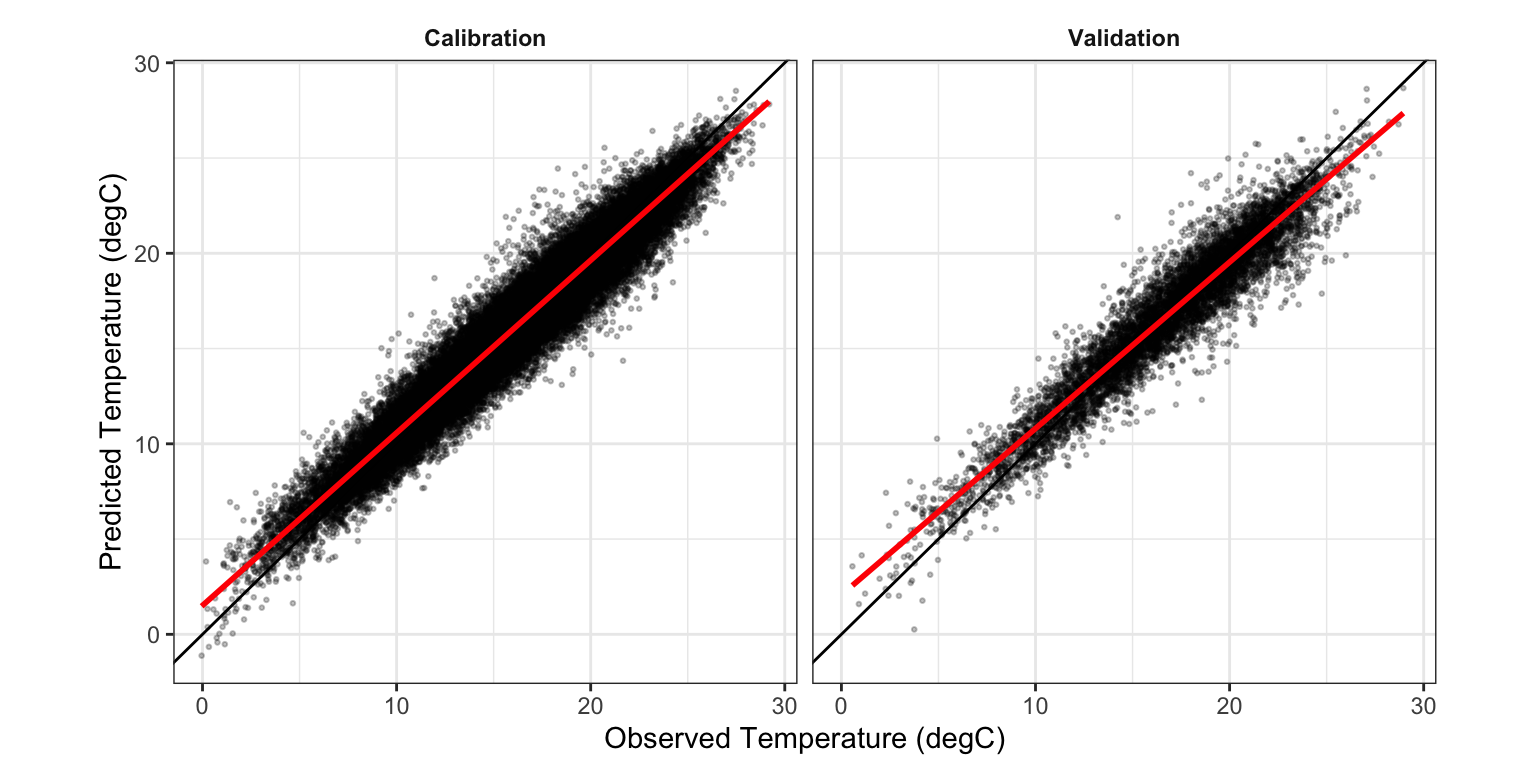
\includegraphics{sheds-temp-model_files/figure-latex/splot-calib-valid-pred-1.pdf}
\caption{\label{fig:splot-calib-valid-pred}Predicted versus Observed Daily Mean Temperature (degC) for Calibration and Validation Datasets}
\end{figure}

\hypertarget{deployments}{%
\subsection{Deployments}\label{deployments}}

Table \ref{tab:table-gof-series} summarises the mean, median, minimum and maximum RMSE for each deployment (i.e.~continuous timeseries of observations at a single location) in the calibration and validation datasets.

\begin{table}

\caption{\label{tab:table-gof-series}Summary statistics of model calibration and validation RMSE for each deployment}
\centering
\begin{tabular}[t]{l|r|r}
\hline
 & Calibration & Validation\\
\hline
\# Time Series & 8495 & 959\\
\hline
Mean RMSE (degC) & 1.043 & 1.345\\
\hline
Median RMSE (degC) & 0.938 & 1.133\\
\hline
Minimum RMSE (degC) & 0.189 & 0.152\\
\hline
Maximum RMSE (degC) & 8.709 & 12.401\\
\hline
\end{tabular}
\end{table}

Figure \ref{fig:plot-hist-series-rmse} shows the distribution of deployment RMSE.

\begin{figure}
\centering
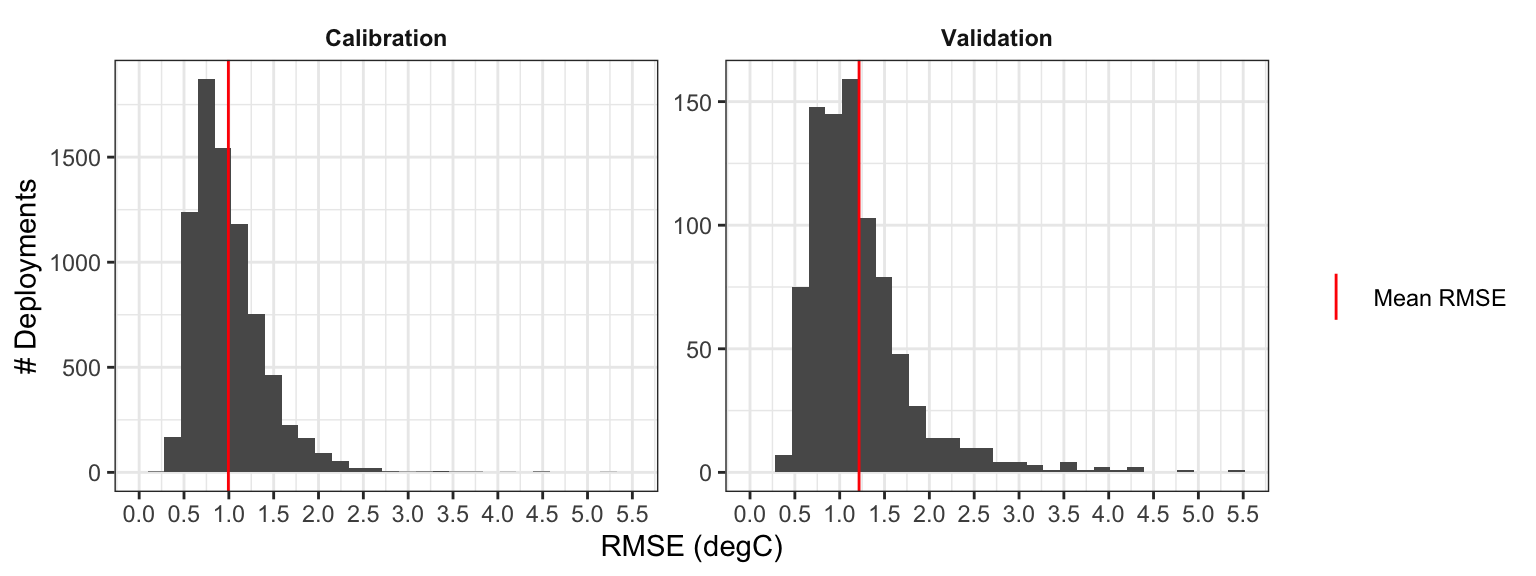
\includegraphics{sheds-temp-model_files/figure-latex/plot-hist-series-rmse-1.pdf}
\caption{\label{fig:plot-hist-series-rmse}Distribution of deployment RMSE}
\end{figure}

\hypertarget{calibration-deployment-examples}{%
\subsubsection{Calibration Deployment Examples}\label{calibration-deployment-examples}}

Figures \ref{fig:plot-series-calib-best} to \ref{fig:plot-series-calib-worst} show example deployments from the calibration dataset with the highest and lowest RMSE.

\begin{figure}
\centering
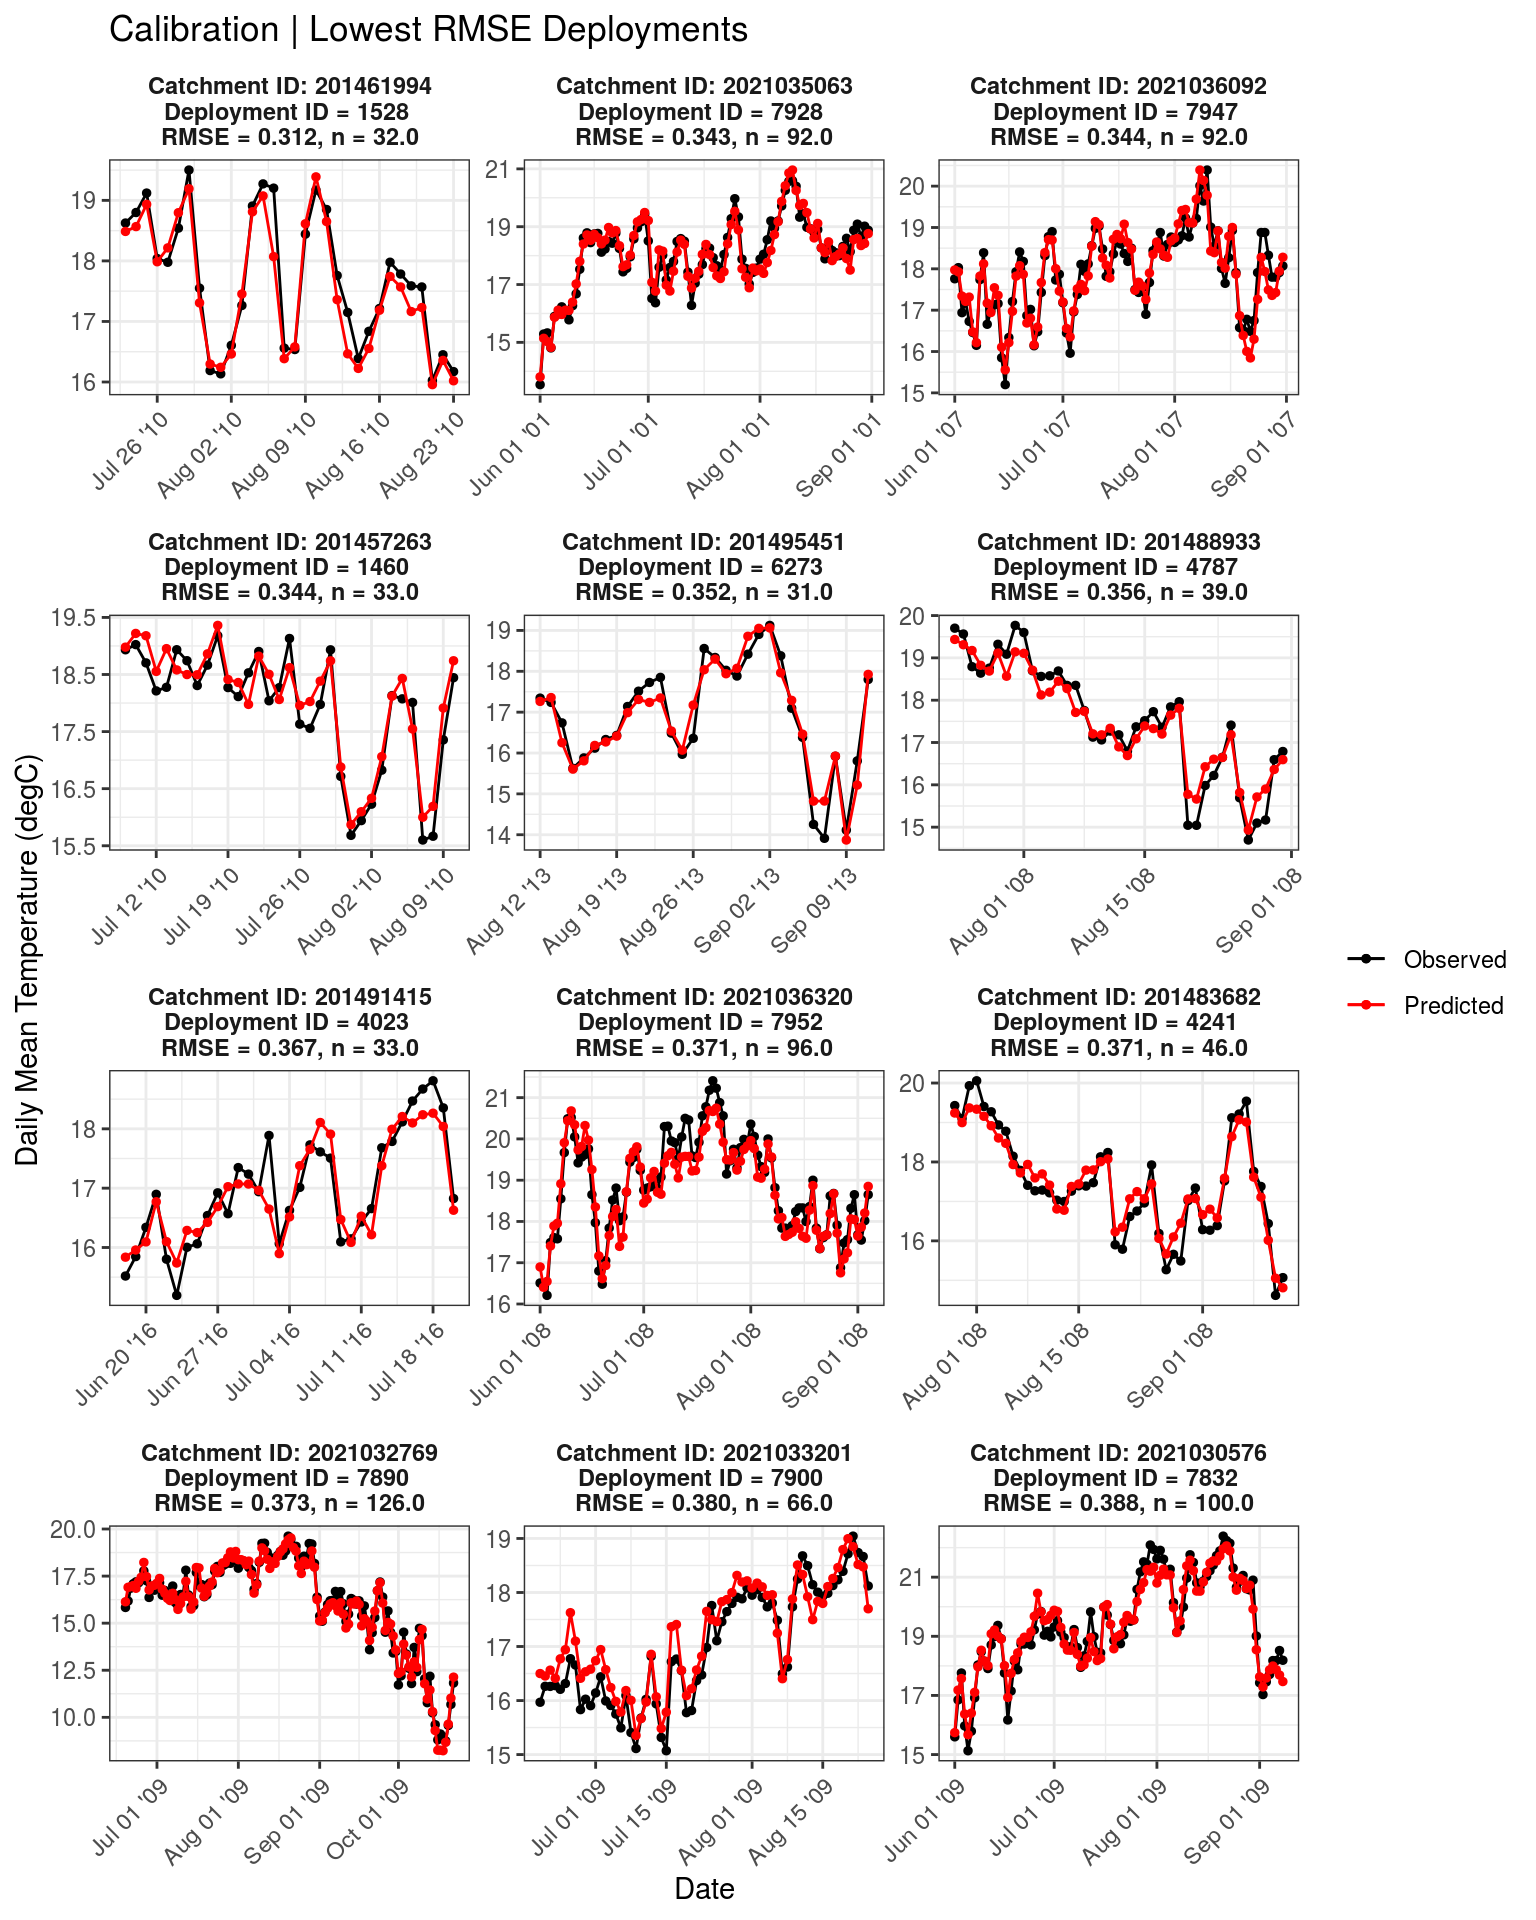
\includegraphics{sheds-temp-model_files/figure-latex/plot-series-calib-best-1.pdf}
\caption{\label{fig:plot-series-calib-best}Deployments with lowest RMSE in calibration dataset and n \textgreater{}= 30}
\end{figure}

\begin{figure}
\centering
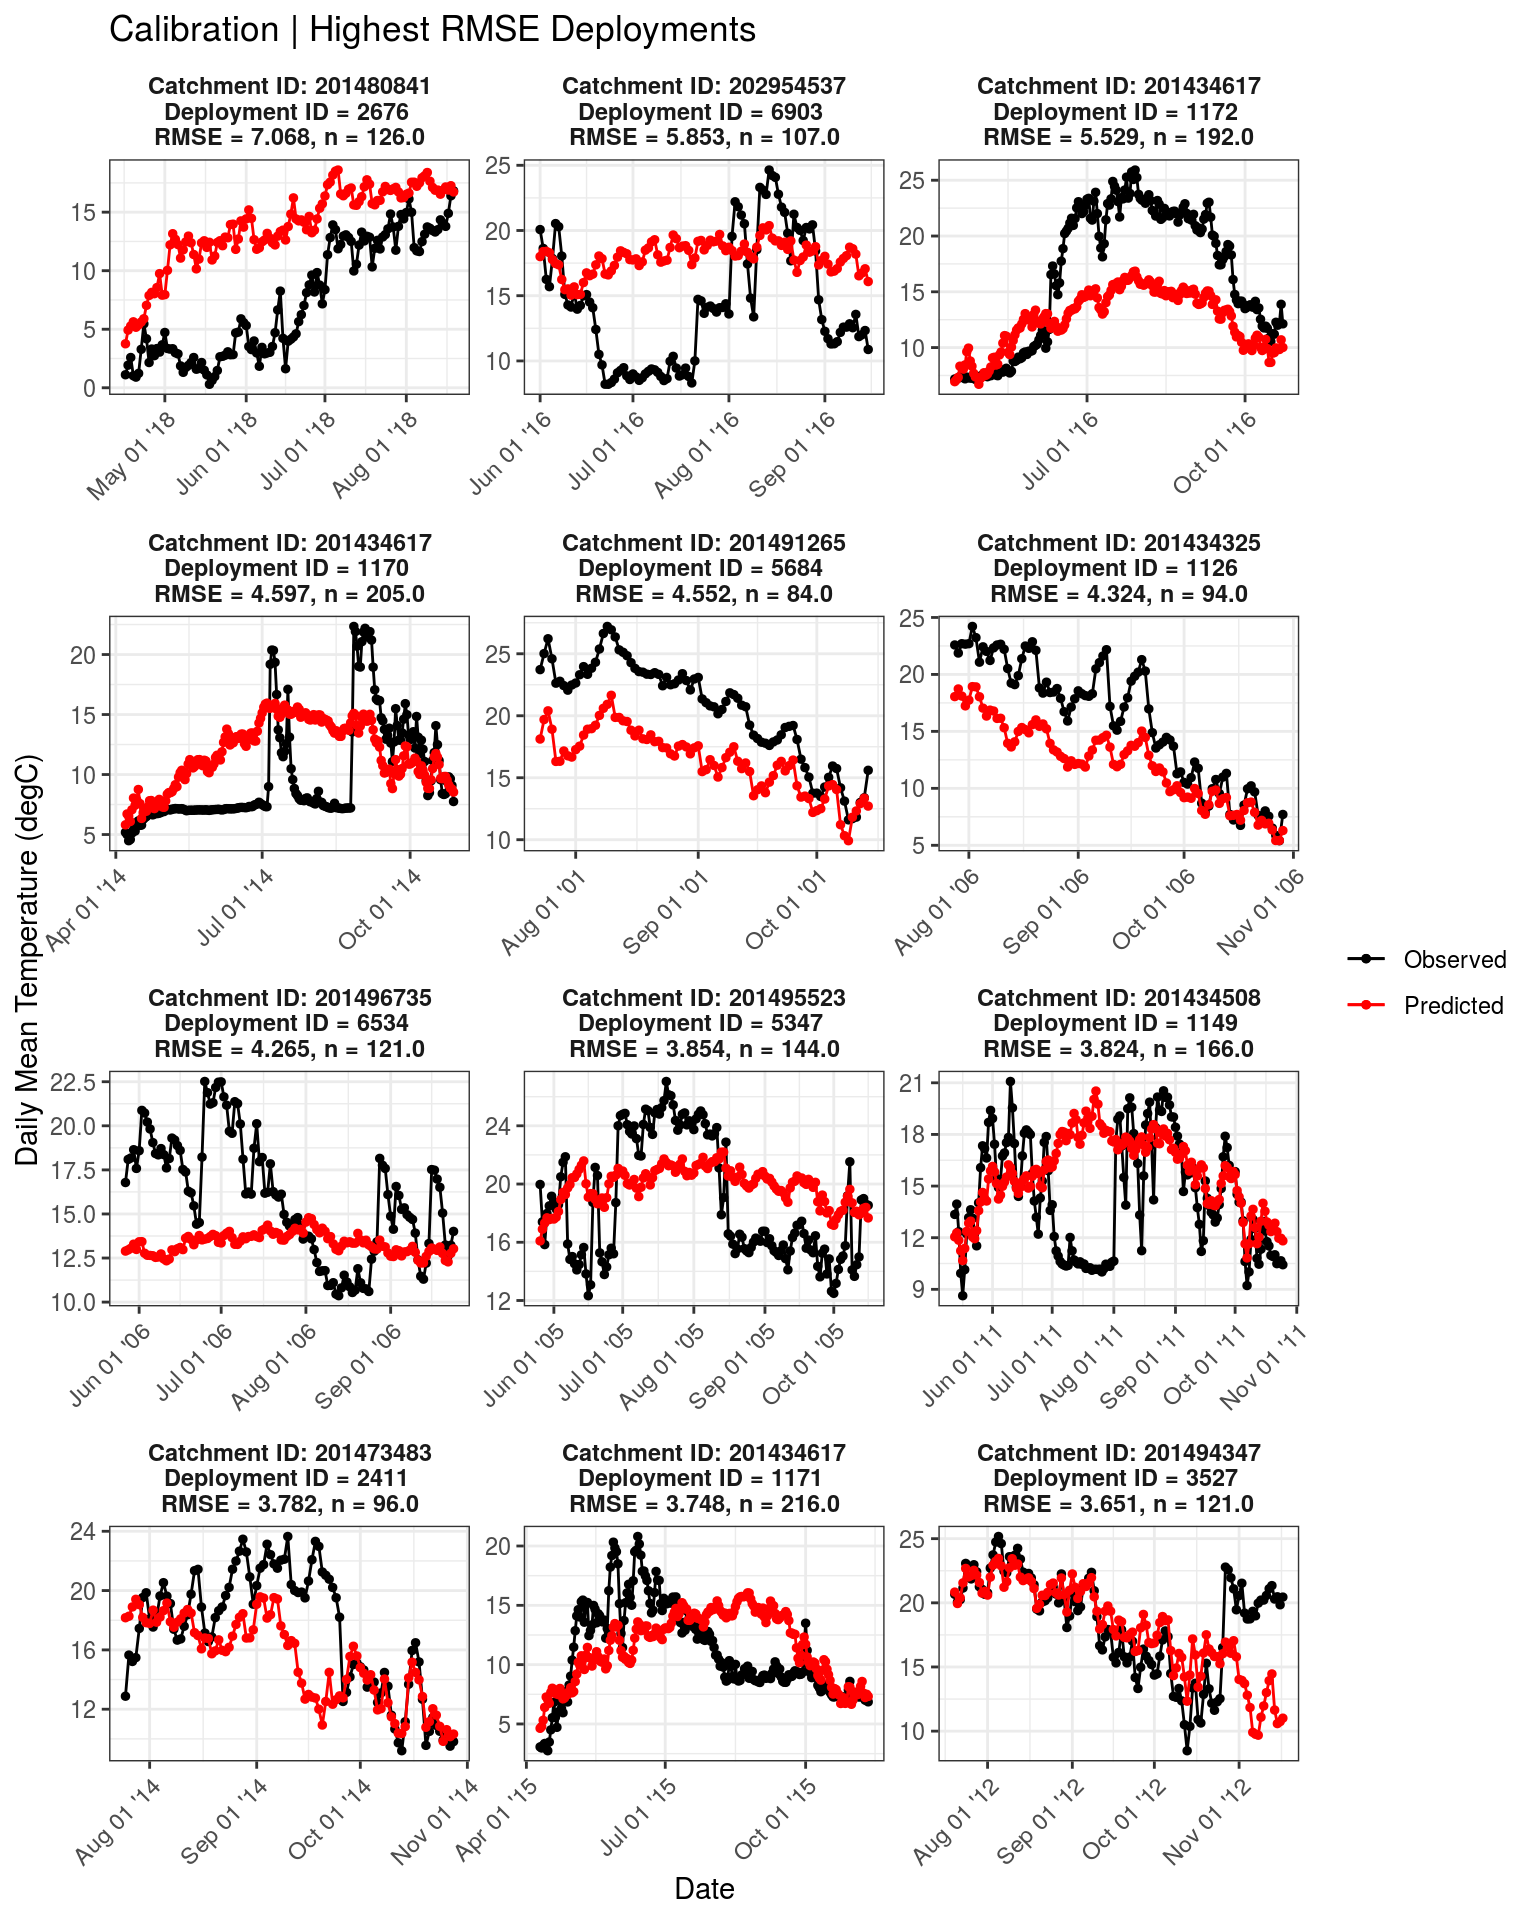
\includegraphics{sheds-temp-model_files/figure-latex/plot-series-calib-worst-1.pdf}
\caption{\label{fig:plot-series-calib-worst}Deployments with highest RMSE in calibration dataset and n \textgreater{}= 30}
\end{figure}

\hypertarget{validation-deployment-examples}{%
\subsubsection{Validation Deployment Examples}\label{validation-deployment-examples}}

Figures \ref{fig:plot-series-valid-best} to \ref{fig:plot-series-valid-worst} show example deployments from the validation dataset with the highest and lowest RMSE.

\begin{figure}
\centering
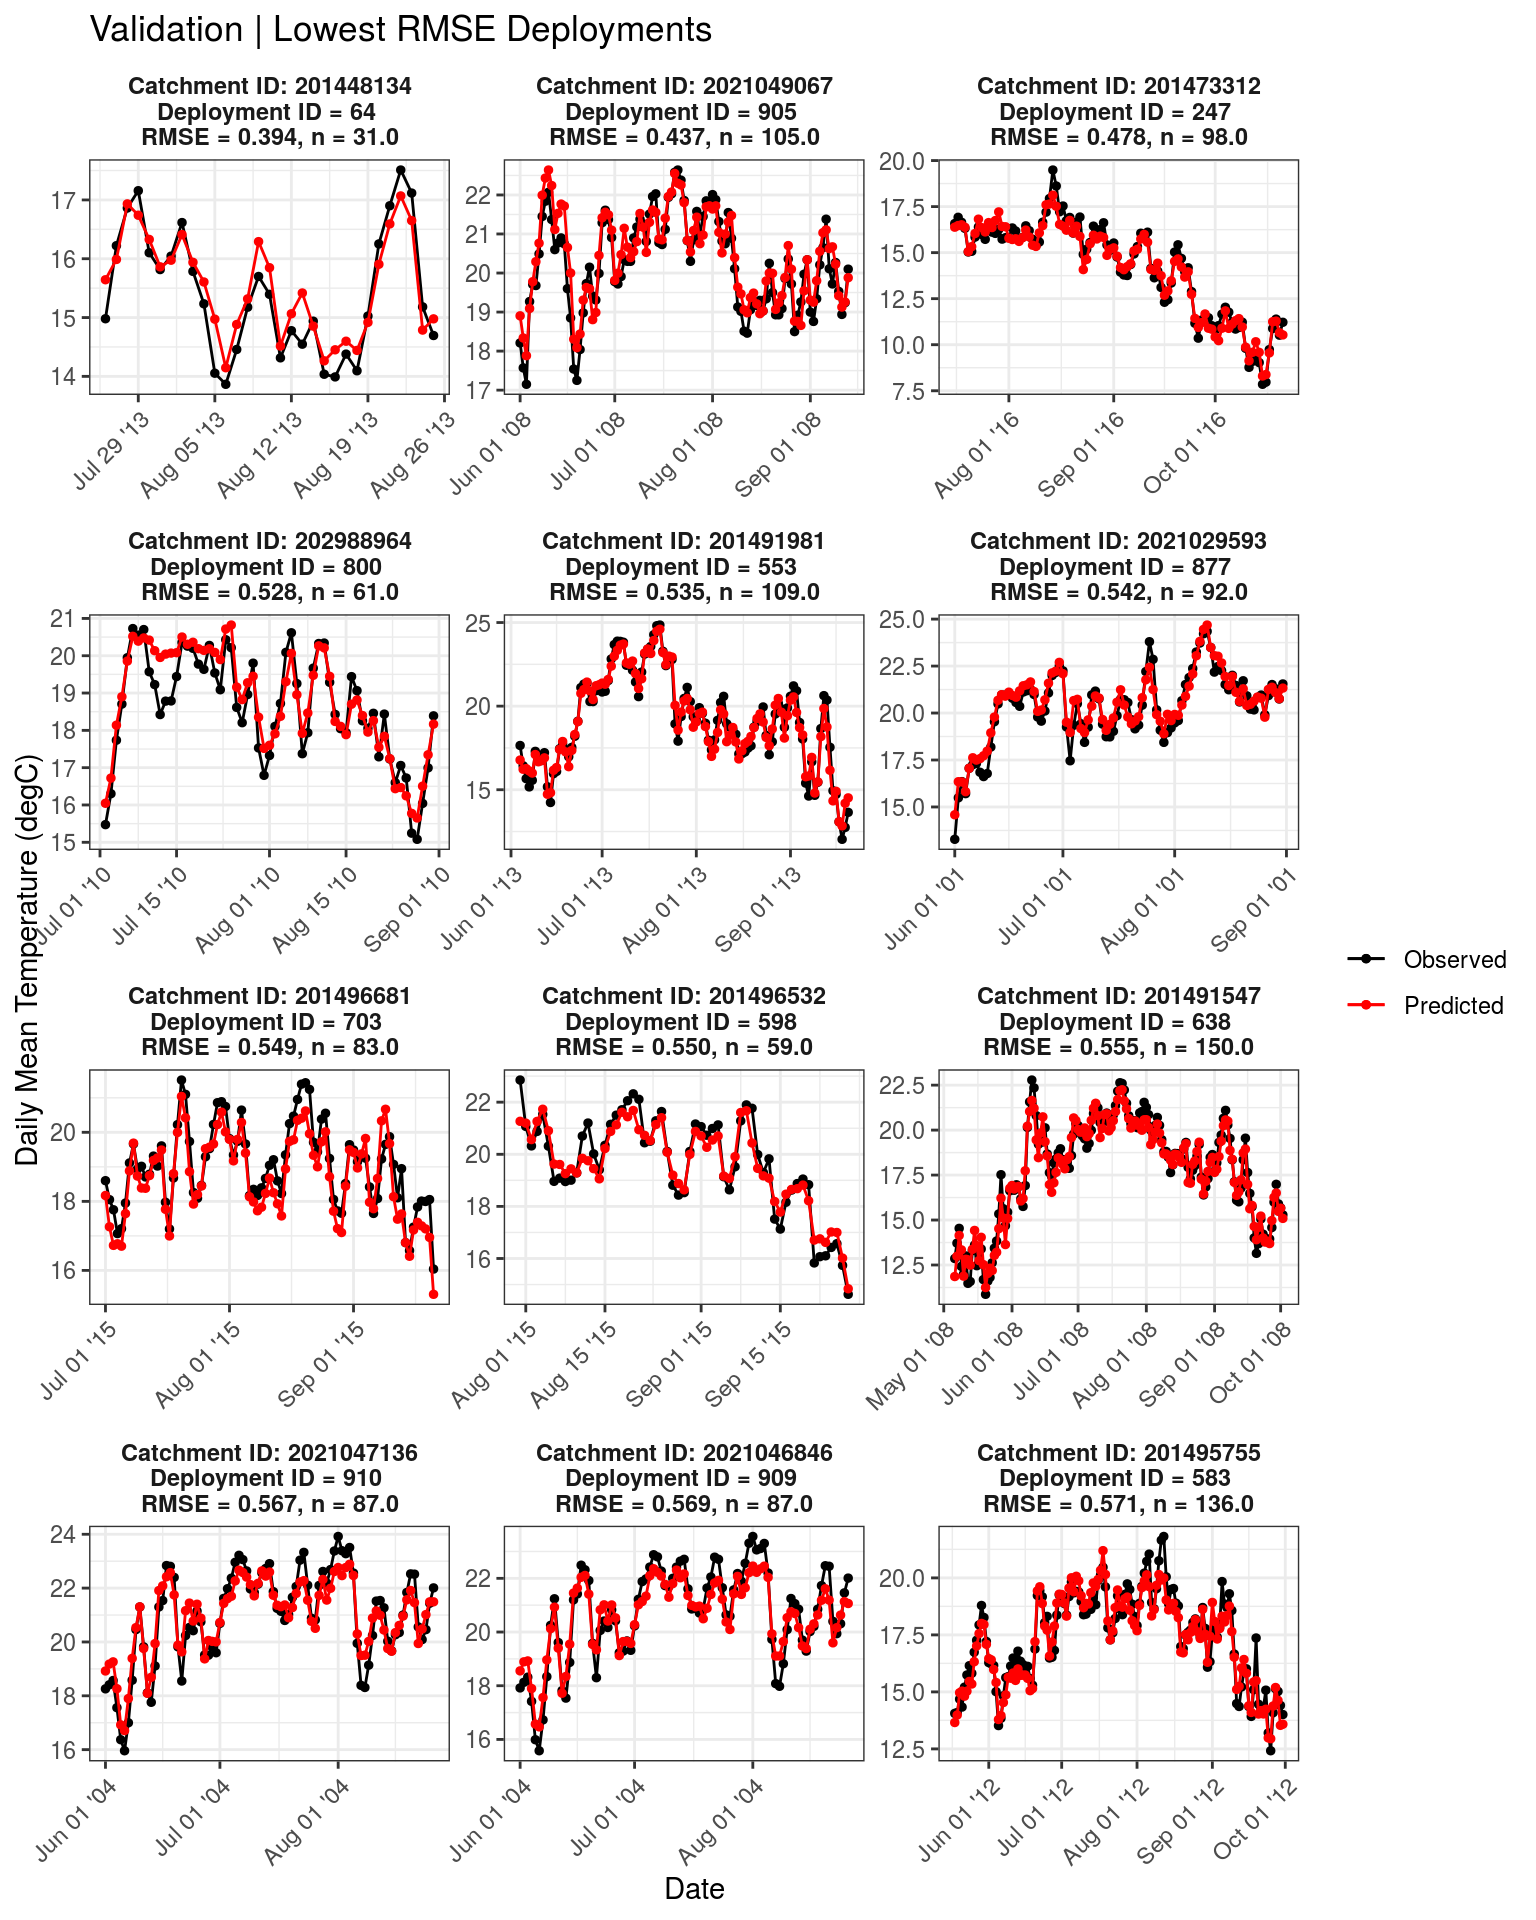
\includegraphics{sheds-temp-model_files/figure-latex/plot-series-valid-best-1.pdf}
\caption{\label{fig:plot-series-valid-best}Deployments with lowest RMSE in validation dataset and n \textgreater{}= 30}
\end{figure}

\begin{figure}
\centering
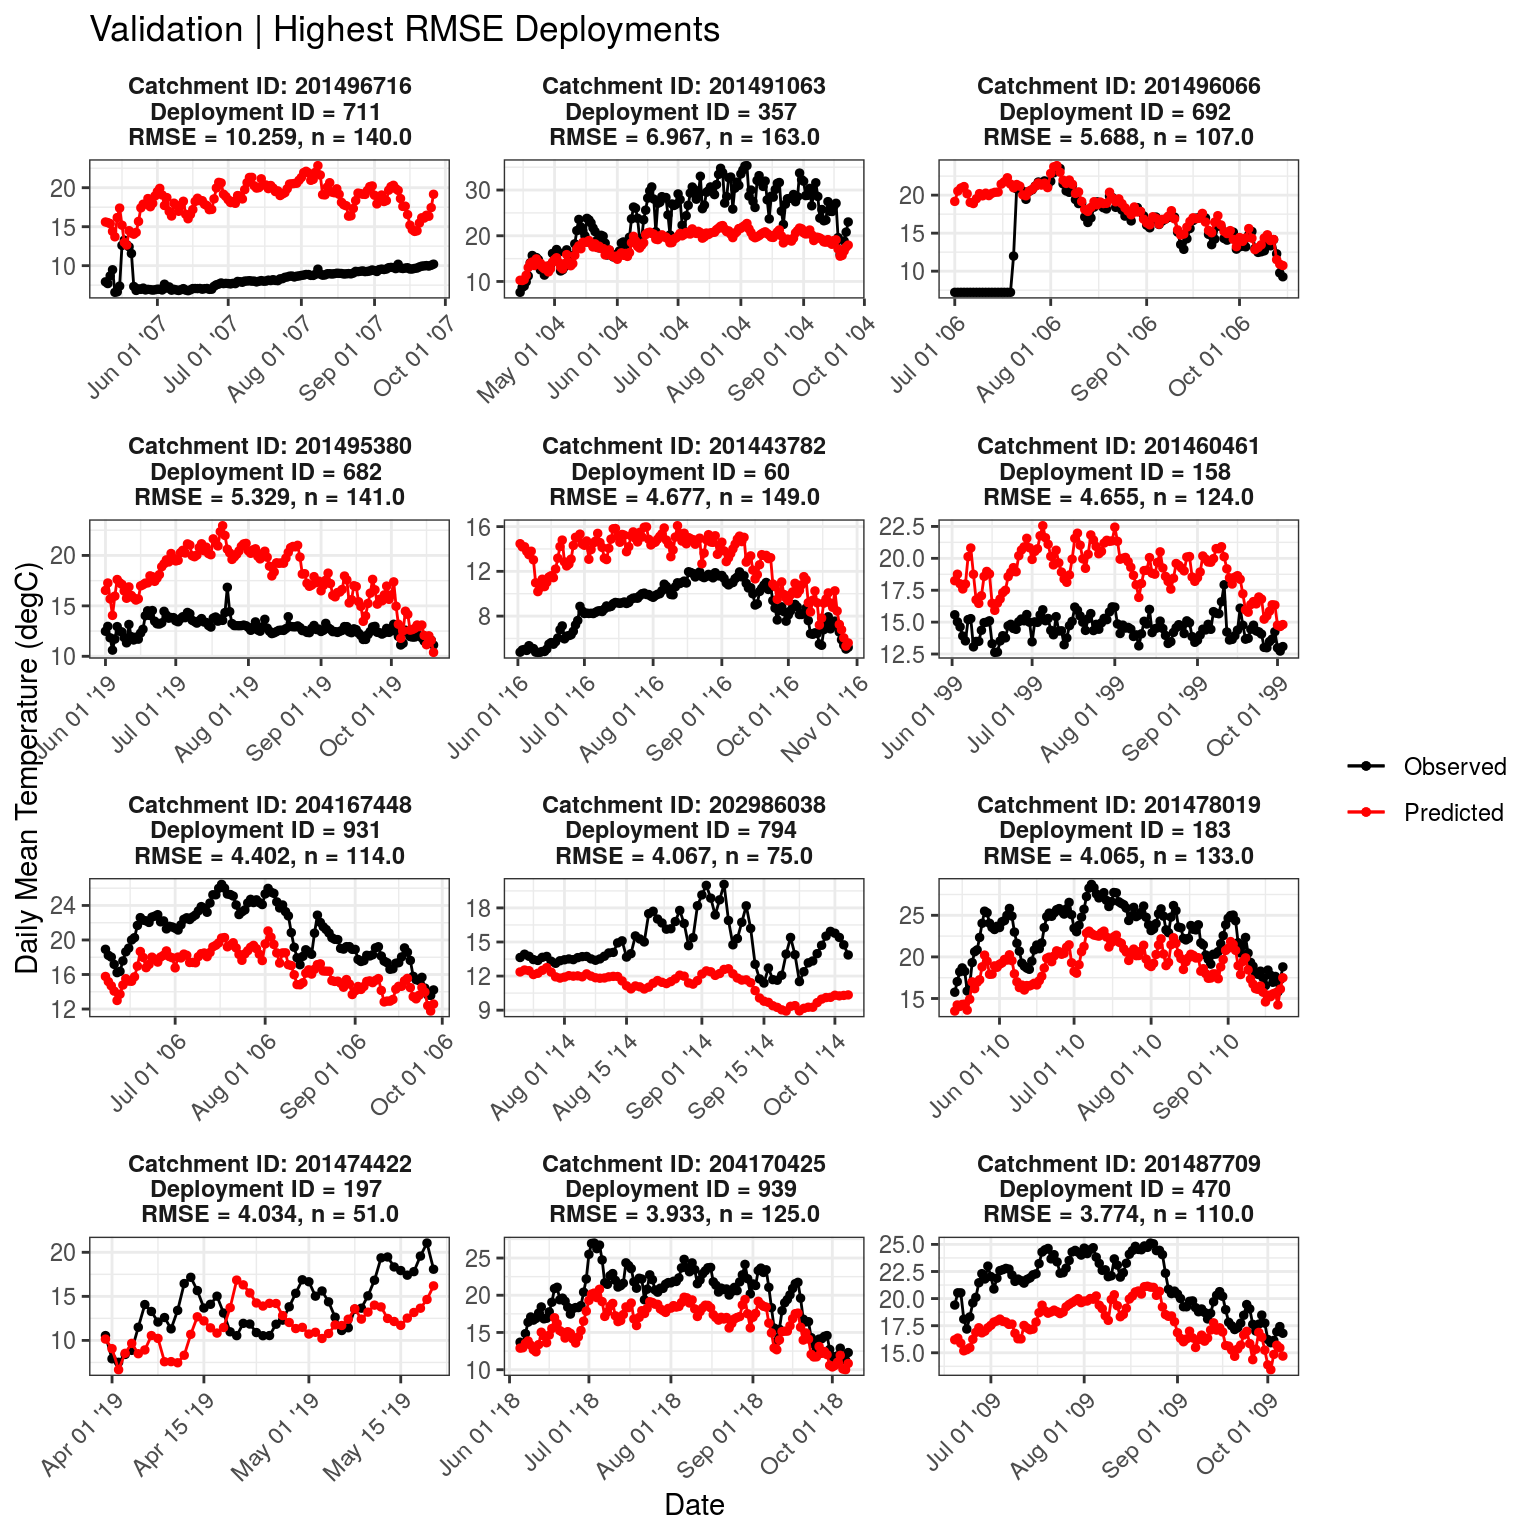
\includegraphics{sheds-temp-model_files/figure-latex/plot-series-valid-worst-1.pdf}
\caption{\label{fig:plot-series-valid-worst}Deployments with highest RMSE in validation dataset and n \textgreater{}= 30}
\end{figure}

\hypertarget{catchments}{%
\subsection{Catchments}\label{catchments}}

Table \ref{tab:table-gof-catchment} summarises the mean, median, minimum and maximum RMSE of all catchments in the calibration and validation datasets.

\begin{table}

\caption{\label{tab:table-gof-catchment}Summary of catchment RMSE values for calibration and validation datasets}
\centering
\begin{tabular}[t]{l|r|r}
\hline
 & Calibration & Validation\\
\hline
\# Time Series & 3077 & 614\\
\hline
Mean RMSE (degC) & 0.970 & 1.436\\
\hline
Median RMSE (degC) & 0.869 & 1.149\\
\hline
Minimum RMSE (degC) & 0.281 & 0.394\\
\hline
Maximum RMSE (degC) & 4.630 & 12.401\\
\hline
\end{tabular}
\end{table}

Figure \ref{fig:plot-hist-catchment-rmse} shows the distribution of catchment RMSE.

\begin{figure}
\centering
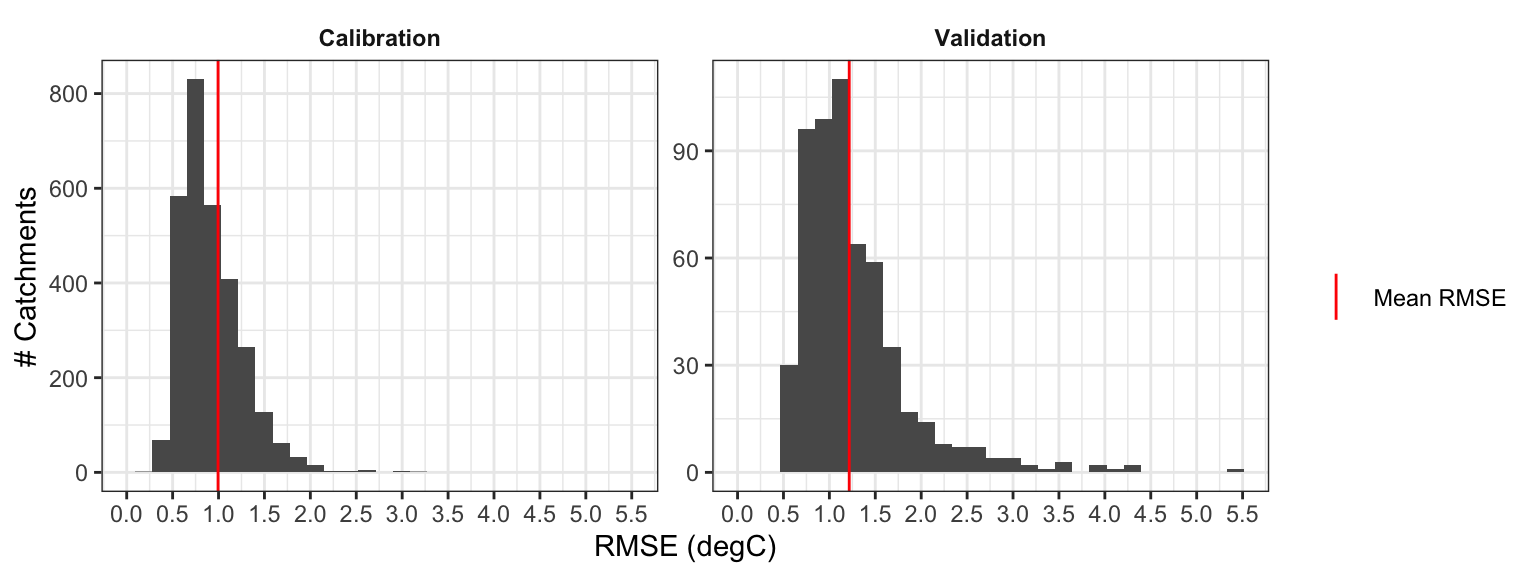
\includegraphics{sheds-temp-model_files/figure-latex/plot-hist-catchment-rmse-1.pdf}
\caption{\label{fig:plot-hist-catchment-rmse}Distribution of catchment RMSE}
\end{figure}

\hypertarget{predictions}{%
\chapter{Predictions}\label{predictions}}

Once calibrated, the model is used to generate stream temperature predictions for all catchments in the region having drainage areas less than 200 sq km and less than 70\% open water coverage.

First, daily time series of predicted mean temperature are generated for each catchment. The daily predictions are then aggregated by year by calculated various metrics such as mean monthly temperatures and frequencies of exceeding various thresholds. Lastly, the annual temperature metrics are aggregated by catchment over all years in the historical period of record.

For each catchment, predictions are generated by the following steps:

\begin{enumerate}
\def\labelenumi{\arabic{enumi}.}
\tightlist
\item
  Calculate the predicted daily mean stream temperature for each year in the historical period of record (1980 - 2020) during the months of June, July and August
\item
  For each month and year, calculate the following metrics:

  \begin{itemize}
  \tightlist
  \item
    Mean monthly temperature (June, July, August)
  \item
    Mean and maximum summer temperature (June 1 - August 31)
  \item
    Maximum 30-day rolling mean temperature
  \item
    Number of days with temperature exceeding 18, 20, and 22 deg C
  \item
    Resistivity computed as the sum of the absolute difference between the predicted stream temperature and the daily mean air temperature (June 1 to August 31)
  \end{itemize}
\item
  For each catchment, the annual metrics from the previous step are aggregated by calculating the following metrics over all years:

  \begin{itemize}
  \tightlist
  \item
    Mean monthly (June, July, August) and summer (June 1 - August 31) temperature
  \item
    Mean and maximum of the annual maximum summer temperature
  \item
    Mean of the annual maximum 30-dy rolling mean temperature
  \item
    Mean number of days per year exceeding 18, 20, and 22 deg C
  \item
    Mean resistivity
  \end{itemize}
\end{enumerate}

Figure \ref{fig:plot-pred-hist} shows the distribution (histogram) of each final metric for all catchments.

\begin{figure}
\centering
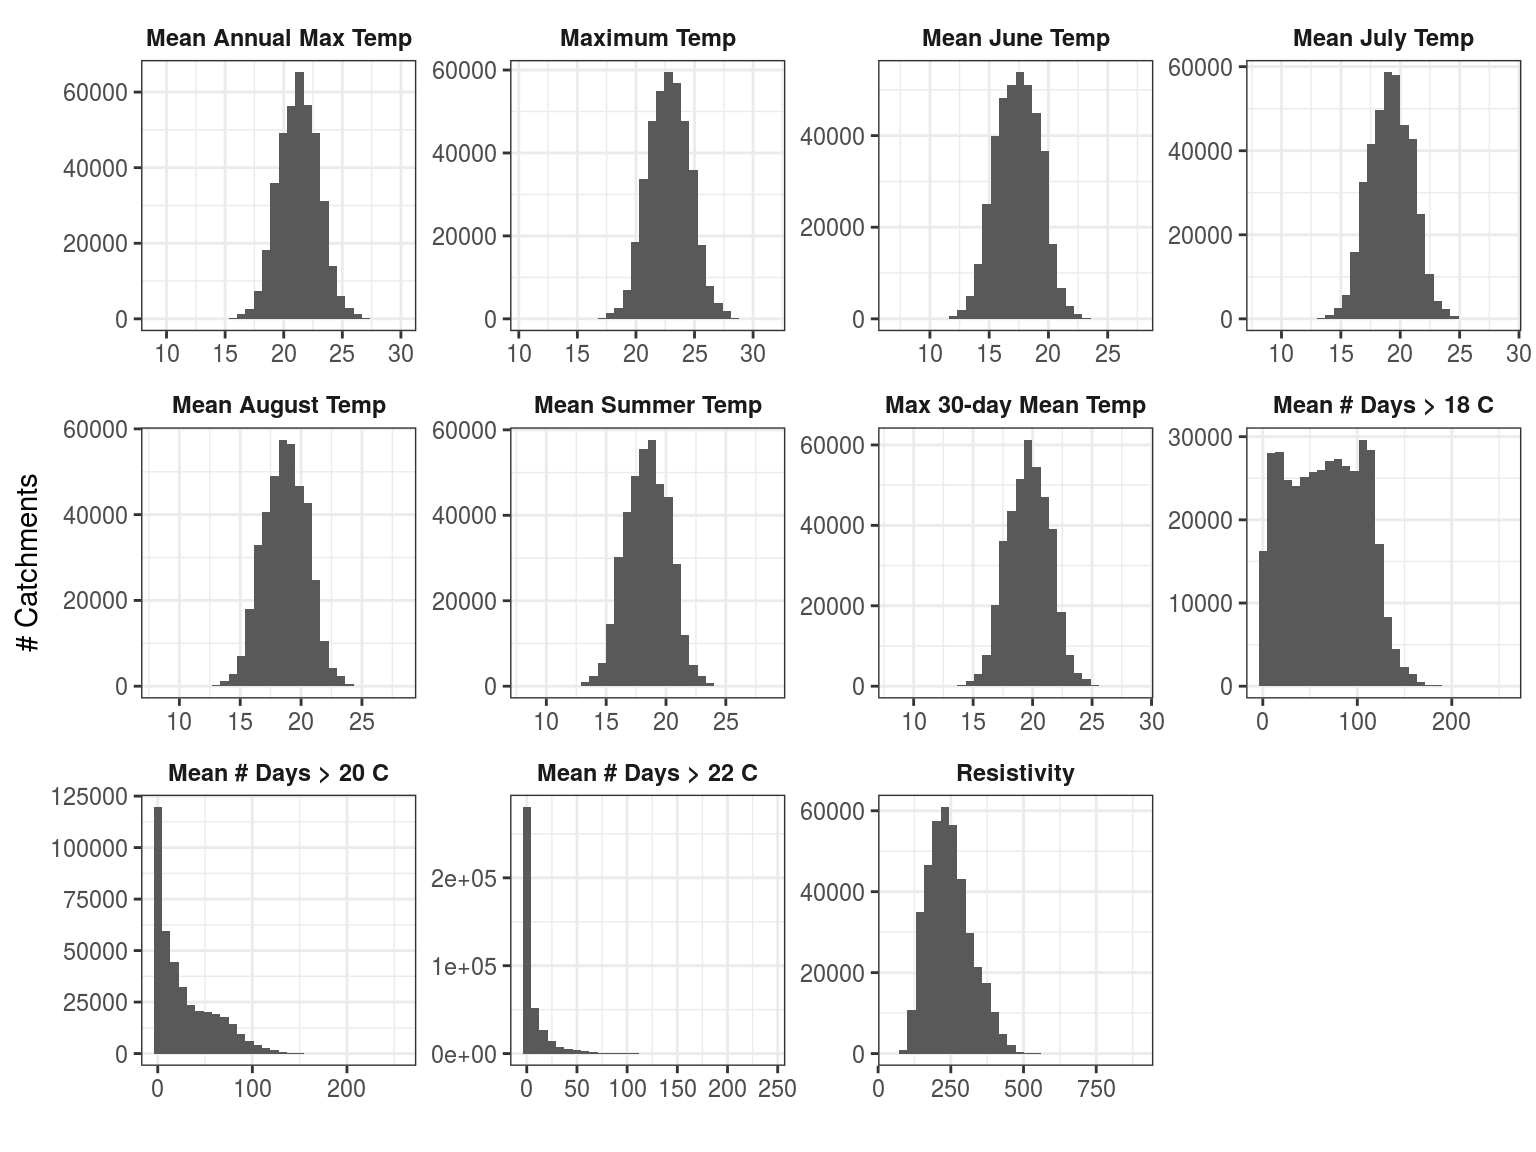
\includegraphics{sheds-temp-model_files/figure-latex/plot-pred-hist-1.pdf}
\caption{\label{fig:plot-pred-hist}Distributions of Catchment Derived Metrics}
\end{figure}

\hypertarget{air-temperature-scenarios}{%
\section{Air Temperature Scenarios}\label{air-temperature-scenarios}}

Beginning with \texttt{v1.1.1}, the prediction metrics described above are generated for a series of climate change scenarios with air temperatures increasing by 2, 4, and 6 degC. These scenarios are calculated by increasing each daily air temperature by the respective amount. In other words, these scenarios assume a uniform increase in air temperature, which does not vary seasonally.

Figure \ref{fig:plot-pred-air-temp} shows the distribution of mean July stream temperature among all catchments for each air temperature scenario.

\begin{figure}
\centering
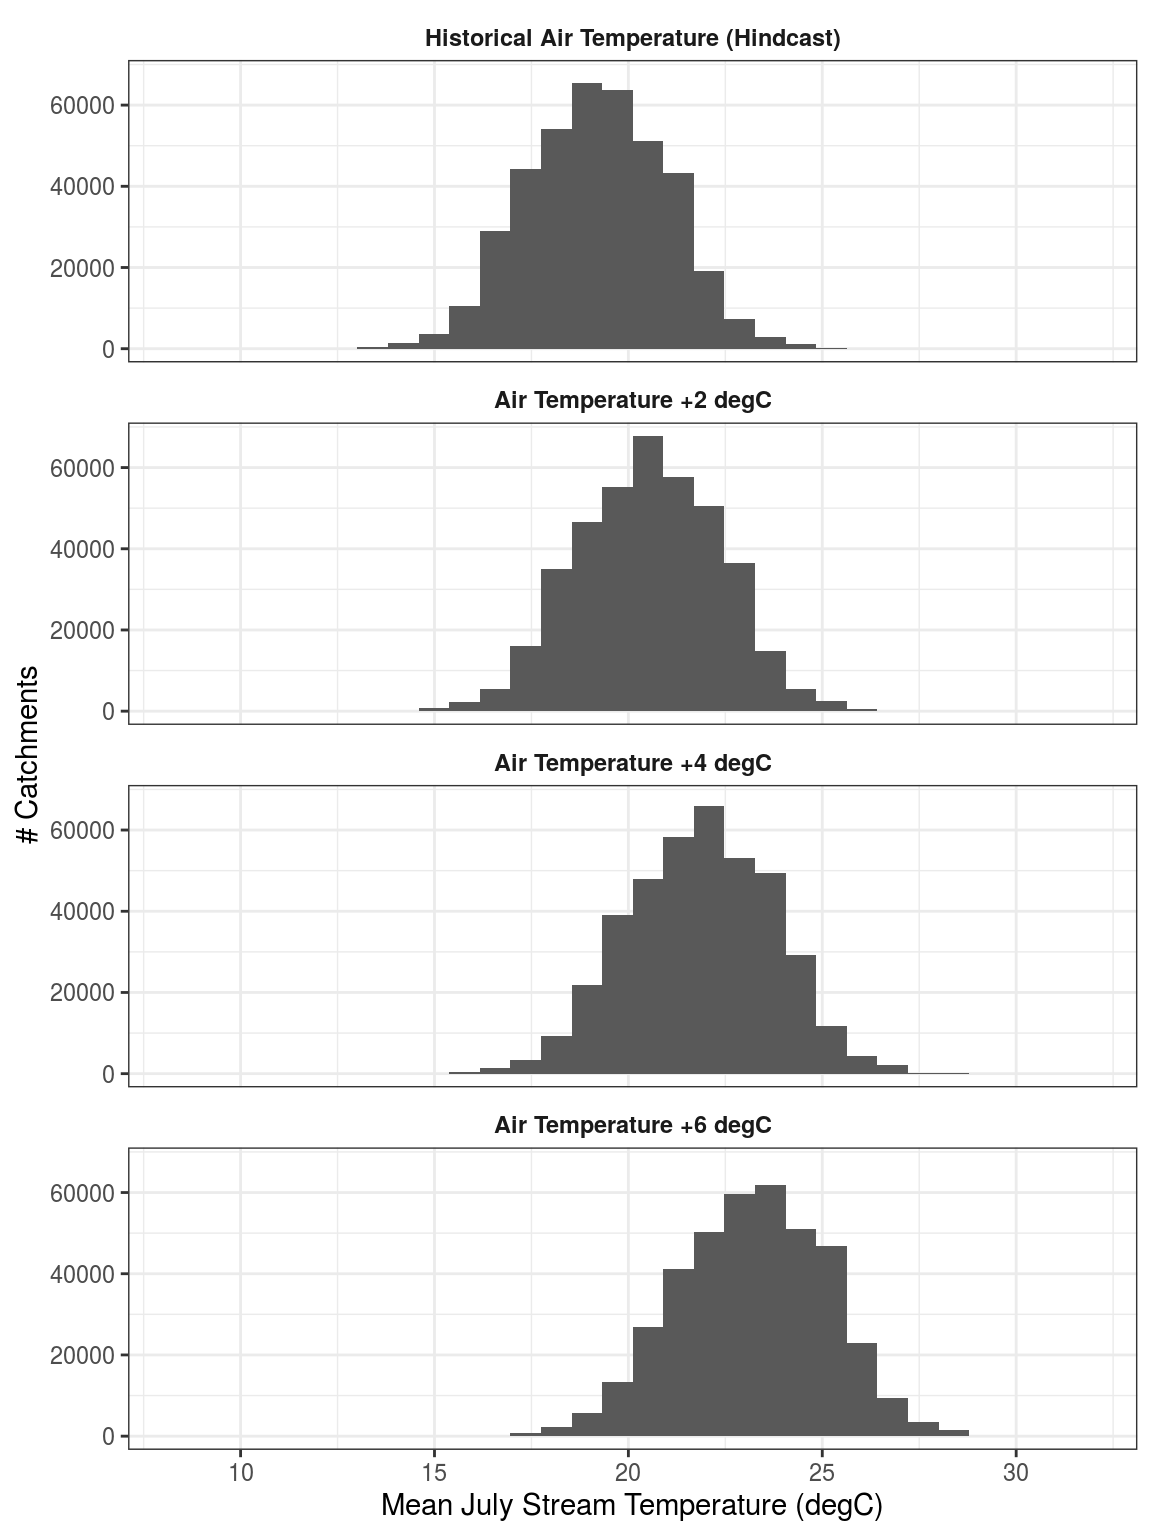
\includegraphics{sheds-temp-model_files/figure-latex/plot-pred-air-temp-1.pdf}
\caption{\label{fig:plot-pred-air-temp}Distributions of Mean July Stream Temperature with Varying Air Temperature Increases}
\end{figure}

\hypertarget{download}{%
\chapter{Download}\label{download}}

\hypertarget{stream-temperature-model-predictions-dataset}{%
\section{Stream Temperature Model Predictions Dataset}\label{stream-temperature-model-predictions-dataset}}

The stream temperature model predictions can be downloaded as a static CSV file from the following link.

\begin{quote}
\textbf{\href{https://ecosheds.org/models/stream-temperature/output/sheds-temp-model-v1.3.0.csv}{Stream Temperature Predictions v1.3.0 (csv)}}
\end{quote}

This file contains the following columns:

\begin{tabular}{r|l}
\hline
CSV Column & Description\\
\hline
featureid & Catchment ID\\
\hline
max\_max\_temp & Maximum Temp (degC)\\
\hline
max\_max\_temp\_air2 & Maximum Temp (degC) w/ Air Temp +2 degC\\
\hline
max\_max\_temp\_air4 & Maximum Temp (degC) w/ Air Temp +4 degC\\
\hline
max\_max\_temp\_air6 & Maximum Temp (degC) w/ Air Temp +6 degC\\
\hline
max\_temp\_30d & Max 30-day Mean Temp (degC)\\
\hline
max\_temp\_30d\_air2 & Max 30-day Mean Temp (degC) w/ Air Temp +2 degC\\
\hline
max\_temp\_30d\_air4 & Max 30-day Mean Temp (degC) w/ Air Temp +4 degC\\
\hline
max\_temp\_30d\_air6 & Max 30-day Mean Temp (degC) w/ Air Temp +6 degC\\
\hline
mean\_aug\_temp & Mean August Temp (degC)\\
\hline
mean\_aug\_temp\_air2 & Mean August Temp (degC) w/ Air Temp +2 degC\\
\hline
mean\_aug\_temp\_air4 & Mean August Temp (degC) w/ Air Temp +4 degC\\
\hline
mean\_aug\_temp\_air6 & Mean August Temp (degC) w/ Air Temp +6 degC\\
\hline
mean\_jul\_temp & Mean July Temp (degC)\\
\hline
mean\_jul\_temp\_air2 & Mean July Temp (degC) w/ Air Temp +2 degC\\
\hline
mean\_jul\_temp\_air4 & Mean July Temp (degC) w/ Air Temp +4 degC\\
\hline
mean\_jul\_temp\_air6 & Mean July Temp (degC) w/ Air Temp +6 degC\\
\hline
mean\_jun\_temp & Mean June Temp (degC)\\
\hline
mean\_jun\_temp\_air2 & Mean June Temp (degC) w/ Air Temp +2 degC\\
\hline
mean\_jun\_temp\_air4 & Mean June Temp (degC) w/ Air Temp +4 degC\\
\hline
mean\_jun\_temp\_air6 & Mean June Temp (degC) w/ Air Temp +6 degC\\
\hline
mean\_max\_temp & Mean Annual Max Temp (degC)\\
\hline
mean\_max\_temp\_air2 & Mean Annual Max Temp (degC) w/ Air Temp +2 degC\\
\hline
mean\_max\_temp\_air4 & Mean Annual Max Temp (degC) w/ Air Temp +4 degC\\
\hline
mean\_max\_temp\_air6 & Mean Annual Max Temp (degC) w/ Air Temp +6 degC\\
\hline
mean\_summer\_temp & Mean Summer Temp (degC)\\
\hline
mean\_summer\_temp\_air2 & Mean Summer Temp (degC) w/ Air Temp +2 degC\\
\hline
mean\_summer\_temp\_air4 & Mean Summer Temp (degC) w/ Air Temp +4 degC\\
\hline
mean\_summer\_temp\_air6 & Mean Summer Temp (degC) w/ Air Temp +6 degC\\
\hline
n\_day\_temp\_gt\_18 & Mean \# Days per Year Temp > 18 C\\
\hline
n\_day\_temp\_gt\_18\_air2 & Mean \# Days per Year Temp > 18 C w/ Air Temp +2 degC\\
\hline
n\_day\_temp\_gt\_18\_air4 & Mean \# Days per Year Temp > 18 C w/ Air Temp +4 degC\\
\hline
n\_day\_temp\_gt\_18\_air6 & Mean \# Days per Year Temp > 18 C w/ Air Temp +6 degC\\
\hline
n\_day\_temp\_gt\_20 & Mean \# Days per Year Temp > 20 C\\
\hline
n\_day\_temp\_gt\_20\_air2 & Mean \# Days per Year Temp > 20 C w/ Air Temp +2 degC\\
\hline
n\_day\_temp\_gt\_20\_air4 & Mean \# Days per Year Temp > 20 C w/ Air Temp +4 degC\\
\hline
n\_day\_temp\_gt\_20\_air6 & Mean \# Days per Year Temp > 20 C w/ Air Temp +6 degC\\
\hline
n\_day\_temp\_gt\_22 & Mean \# Days per Year Temp > 22 C\\
\hline
n\_day\_temp\_gt\_22\_air2 & Mean \# Days per Year Temp > 22 C w/ Air Temp +2 degC\\
\hline
n\_day\_temp\_gt\_22\_air4 & Mean \# Days per Year Temp > 22 C w/ Air Temp +4 degC\\
\hline
n\_day\_temp\_gt\_22\_air6 & Mean \# Days per Year Temp > 22 C w/ Air Temp +6 degC\\
\hline
n\_day\_temp\_gte\_24\_9 & Mean \# Days per Year Temp >= 24.9 C\\
\hline
n\_day\_temp\_gte\_24\_9\_air2 & Mean \# Days per Year Temp >= 24.9 C w/ Air Temp +2 degC\\
\hline
n\_day\_temp\_gte\_24\_9\_air4 & Mean \# Days per Year Temp >= 24.9 C w/ Air Temp +4 degC\\
\hline
n\_day\_temp\_gte\_24\_9\_air6 & Mean \# Days per Year Temp >= 24.9 C w/ Air Temp +6 degC\\
\hline
n\_day\_temp\_gte\_27 & Mean \# Days per Year Temp >= 27 C\\
\hline
n\_day\_temp\_gte\_27\_air2 & Mean \# Days per Year Temp >= 27 C w/ Air Temp +2 degC\\
\hline
n\_day\_temp\_gte\_27\_air4 & Mean \# Days per Year Temp >= 27 C w/ Air Temp +4 degC\\
\hline
n\_day\_temp\_gte\_27\_air6 & Mean \# Days per Year Temp >= 27 C w/ Air Temp +6 degC\\
\hline
resist & Resistivity\\
\hline
resist\_air2 & Resistivity w/ Air Temp +2 degC\\
\hline
resist\_air4 & Resistivity w/ Air Temp +4 degC\\
\hline
resist\_air6 & Resistivity w/ Air Temp +6 degC\\
\hline
\end{tabular}

\hypertarget{catchment-delineation-shapefiles}{%
\section{Catchment Delineation Shapefiles}\label{catchment-delineation-shapefiles}}

The \href{https://conte-ecology.github.io/shedsGisData/}{SHEDS catchment delineation} (NHDHRDV2) are available as a series of shapefiles, pre-staged by 2-digit hydrologic unit codes (HUCs). The model predictions and covariates CSV files can be joined to these shapefiles using the mutual \texttt{featureid} column.

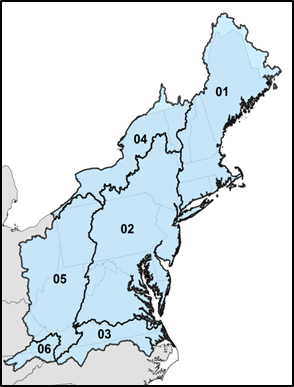
\includegraphics{img/hydrologic-regions.png}

\begin{itemize}
\tightlist
\item
  \href{https://ecosheds.org/assets/nhdhrd/v2/spatial_01.zip}{Region 01 Catchments (zipped shp)}
\item
  \href{https://ecosheds.org/assets/nhdhrd/v2/spatial_02.zip}{Region 02 Catchments (zipped shp)}
\item
  \href{https://ecosheds.org/assets/nhdhrd/v2/spatial_03.zip}{Region 03 Catchments (zipped shp)}
\item
  \href{https://ecosheds.org/assets/nhdhrd/v2/spatial_04.zip}{Region 04 Catchments (zipped shp)}
\item
  \href{https://ecosheds.org/assets/nhdhrd/v2/spatial_05.zip}{Region 05 Catchments (zipped shp)}
\item
  \href{https://ecosheds.org/assets/nhdhrd/v2/spatial_06.zip}{Region 06 Catchments (zipped shp)}
\end{itemize}

The documentation for the catchment delineation is also available:

\begin{quote}
\textbf{\href{https://ecosheds.org/assets/nhdhrd/v2/NHDHRDV2_Documentation.docx}{Catchment Delineation (NHDHRDV2) Documentation (docx)}}
\end{quote}

\hypertarget{catchment-covariates-dataset}{%
\section{Catchment Covariates Dataset}\label{catchment-covariates-dataset}}

The \href{https://conte-ecology.github.io/shedsGisData/}{SHEDS catchment covariates} are available as a series of CSV files, pre-staged by 2-digit hydrologic unit codes (HUCs). The covariates contain the catchment characteristics that are used as input variables to the stream temperature model.

\begin{itemize}
\tightlist
\item
  \href{https://ecosheds.org/assets/nhdhrd/v2/covariates_01.zip}{Region 01 Covariates (zipped csv)}
\item
  \href{https://ecosheds.org/assets/nhdhrd/v2/covariates_02.zip}{Region 02 Covariates (zipped csv)}
\item
  \href{https://ecosheds.org/assets/nhdhrd/v2/covariates_03.zip}{Region 03 Covariates (zipped csv)}
\item
  \href{https://ecosheds.org/assets/nhdhrd/v2/covariates_04.zip}{Region 04 Covariates (zipped csv)}
\item
  \href{https://ecosheds.org/assets/nhdhrd/v2/covariates_05.zip}{Region 05 Covariates (zipped csv)}
\item
  \href{https://ecosheds.org/assets/nhdhrd/v2/covariates_06.zip}{Region 06 Covariates (zipped csv)}
\end{itemize}

The documentation for catchment covariates is also available:

\begin{quote}
\textbf{\href{https://ecosheds.org/assets/nhdhrd/v2/NHDHRDV2_Covariate_Documentation.xlsx}{Catchment Covariates Documentation (docx)}}
\end{quote}

\hypertarget{references}{%
\chapter*{References}\label{references}}
\addcontentsline{toc}{chapter}{References}

\bibliography{book.bib}

\end{document}
